% !TeX program = pdflatex
% =============================================================
% Public Economics -- Lecture 4
% Taxation (v2)
% Based on: Gruber, J. "Public Finance and Public Policy", Ch. 18-22
%           Leenders, W. "Microeconomics of Public Policy, Part IV:
%           Taxation" (Sciences Po, MPA 2023-2024)
% Austrian institutional and empirical context added for WU Vienna.
% v2: extended with material from a colleague's parallel WU course
%     (Edoardo Cefala, Slides_Edoardo/), inserted where topically
%     relevant. Original structure preserved; nothing removed.
% =============================================================
\documentclass[11pt,aspectratio=169]{beamer}

\usetheme{metropolis}
\usepackage[utf8]{inputenc}
\usepackage[T1]{fontenc}
\usepackage{lmodern}
\usepackage{booktabs}
\usepackage{array}
\usepackage{textcomp}
\usepackage{siunitx}
\usepackage{tikz}
\usepackage{pgfplots}
\pgfplotsset{compat=1.18}
\usepackage{pgf-pie}
\usetikzlibrary{positioning,arrows.meta,calc}
\usepackage{eso-pic}

% ----------------------------------------------------------------
% Colors: WU Vienna blue as primary accent
% ----------------------------------------------------------------
\definecolor{wublue}{HTML}{003D7C}
\definecolor{wulight}{HTML}{4F8FC4}
\definecolor{wugray}{HTML}{5C6670}
\definecolor{wured}{HTML}{B0202E}
\definecolor{wugreen}{HTML}{4C8C6B}
\definecolor{wuyellow}{HTML}{D9A441}
\setbeamercolor{palette primary}{bg=wublue,fg=white}
\setbeamercolor{frametitle}{bg=wublue,fg=white}
\setbeamercolor{progress bar}{fg=wublue,bg=wulight!30}
\setbeamercolor{alerted text}{fg=wured}

\setbeamertemplate{frame footer}{Taxation}
\setbeamertemplate{footline}[frame number]

\title{Public Economics}
\subtitle{ \(\cdot\) Taxation}
\author{Shushanik Margaryan}
\institute{WU Vienna University of Economics and Business}
\titlegraphic{
\includegraphics[height=1.0cm]{../assets/wu_logo.png}}
\date{Winter Term}

% Source note command for footnote-style citations on data slides
\newcommand{\srcnote}[1]{{\footnotesize\color{wugray}Source: #1}}

\begin{document}

% =============================================================
\begin{frame}
  \titlepage
\end{frame}

\AddToShipoutPictureFG{%
  \AtPageUpperLeft{%
    \put(\LenToUnit{\paperwidth-2.0cm},\LenToUnit{-0.85cm}){
\includegraphics[height=0.62cm]{../assets/wu_logo_white.png}}%
  }%
}

\begin{frame}{Today's Questions}
  \begin{itemize}
    \item What are the different types of taxes governments levy, and how does the burden of a tax actually get shared between buyers and sellers?
    \item What does it mean for a tax system to be ``fair,'' and how do we measure that?

  \end{itemize}
  \vspace{1em}
  \begin{block}{Based on}
    Gruber, J. \emph{Public Finance and Public Policy}, Ch.\ 18
  \end{block}
\end{frame}

% =============================================================
\begin{frame}{Outline}
  \tableofcontents
\end{frame}

% =============================================================
\section{4.1 Types of Taxation}

\begin{frame}{Five Types of Taxes}
  \small
  \begin{itemize}
    \item \textbf{Payroll tax}: levied on earnings from work; finances social insurance (pensions, unemployment, health).
    \item \textbf{Individual income tax}: paid on income accrued during the year --- a broader base than payroll (interest, etc.) and often assessed per household, not per worker.
    \item \textbf{Corporate income tax}: levied on corporate earnings, to catch capital income that might otherwise escape individual-level taxation.
    \item \textbf{Wealth taxes}: levied on the \emph{value of assets} held (not income), e.g.\ property tax, estate/inheritance tax.
    \item \textbf{Consumption taxes}: levied on spending, e.g.\ VAT/sales tax; when applied to one specific good (fuel, tobacco, alcohol), called an \textbf{excise tax}.
  \end{itemize}
  \vspace{0.3em}
  \centering

\end{frame}

\begin{frame}{The Same Five Types, in Austria}
  \scriptsize
  \begin{center}
  \begin{tabular}{@{}p{2.6cm}p{9.3cm}@{}}
    \toprule
    \textbf{Type} & \textbf{Austrian tax(es)} \\
    \midrule
    Payroll & \emph{Sozialversicherungsbeiträge} --- pension, health, unemployment, accident insurance; split employer/employee \\[0.2em]
    Individual income & \emph{Einkommensteuer} (self-employment/business income); \emph{Lohnsteuer} (withholding on wage income) \\[0.2em]
    Corporate income & \emph{Körperschaftsteuer} (KSt) \\[0.2em]
    Wealth & \emph{Grundsteuer} (property) and \emph{Grunderwerbsteuer} (real-estate transfer) still exist; \emph{Vermögensteuer} and \emph{Erbschafts-/Schenkungssteuer} do \textbf{not} \\[0.2em]
    Consumption & \emph{Umsatzsteuer} (VAT); excise: \emph{Mineralölsteuer} (fuel), \emph{Tabaksteuer}, \emph{Alkohol-/Biersteuer}, \emph{NoVA} (vehicles), \emph{CO\textsubscript{2}-Bepreisung} (since 2022) \\
    \bottomrule
  \end{tabular}
  \end{center}
  \centering

\end{frame}

\begin{frame}{International Tax Revenues by Type}
\centering



		\textbf{OECD average}\\[0.2em]
			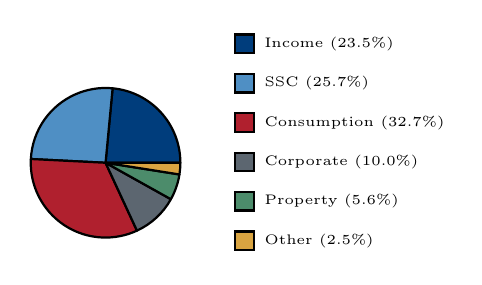
\begin{tikzpicture}
				\pie[
				radius=0.95, text=legend, hide number, font=\tiny,
				color={wublue,wulight,wured,wugray,wugreen,wuyellow}
				]{
					23.5/Income (23.5\%),
					25.7/SSC (25.7\%),
					32.7/Consumption (32.7\%),
					10.0/Corporate (10.0\%),
					5.6/Property (5.6\%),
					2.5/Other (2.5\%)
				}
			\end{tikzpicture}

\end{frame}

\begin{frame}{Taxation Around the World: Tax Revenue Composition}
  \begin{center}
   % 
\includegraphics[height=4.55cm]{figures/taxation_around_world_norway_denmark_oecd.png}
  \end{center}
  \centering
  Two very different high-tax countries: Norway spreads revenue broadly across income, payroll, and corporate taxes; Denmark relies overwhelmingly on the individual income tax alone.\\
  \srcnote{Gruber, \emph{Public Finance and Public Policy}, \S18.1, ``Taxation Around the World.''}
\end{frame}

\begin{frame}{Where Does Austria Fit?}
  \begin{itemize}
    \item  Austria's tax mix leans heavily on \textbf{labor}
    \item  Austria abolished its general \textbf{wealth tax} (\emph{Vermögensteuer}) in 1994, and its \textbf{inheritance/gift tax} lapsed in 2008 after the \emph{Verfassungsgerichtshof} ruled the property-valuation method unconstitutional and no replacement was passed.
    \item Austria has had \emph{no} wealth or inheritance tax since.
  \end{itemize}

\end{frame}

% =============================================================
\section{4.2 Tax Incidence}

\begin{frame}{Tax Incidence: Who Really Pays?}
  \begin{block}{Tax incidence}
   Tax incidence measures who bears the legal or economic burden of a tax.
  \end{block}
  \vspace{0.3em}
  \begin{itemize}
    \item \textbf{Legal (statutory) incidence}: who is legally required to send the tax payment to the government.
    \item \textbf{Economic incidence}: who actually bears the burden, once prices adjust.
  \end{itemize}


\end{frame}

\begin{frame}{The Canonical Case: An Excise Tax}
  \begin{center}
  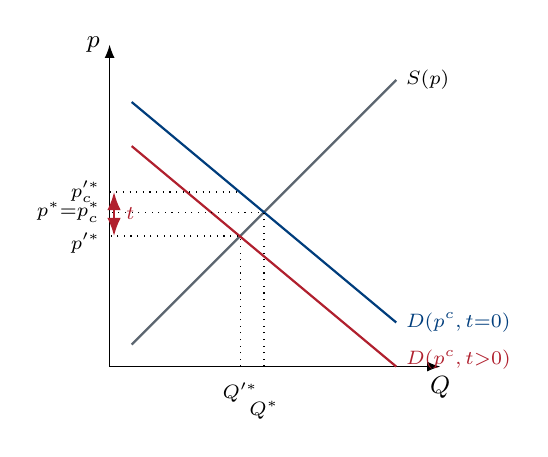
\begin{tikzpicture}[scale=0.56]
    \draw[-{Latex}] (0,0) -- (7.5,0) node[below, font=\small]{$Q$};
    \draw[-{Latex}] (0,0) -- (0,7.3) node[left, font=\small]{$p$};
    \draw[wugray, thick] (0.5,0.5) -- (6.5,6.5);
    \node[right, font=\scriptsize] at (6.5,6.5) {$S(p)$};
    \draw[wublue, thick] (0.5,6) -- (6.5,1);
    \node[right, font=\scriptsize, wublue] at (6.5,1) {$D(p^c,t{=}0)$};
    \draw[wured, thick] (0.5,5) -- (6.5,0);
    \node[right, font=\scriptsize, wured] at (6.5,0.15) {$D(p^c,t{>}0)$};
    \draw[dotted] (3.5,0) -- (3.5,3.5) -- (0,3.5);
    \draw[dotted] (2.96,0) -- (2.96,2.96) -- (0,2.96);
    \draw[dotted] (0,3.96) -- (2.96,3.96);
    \draw[wured, thick, {Latex}-{Latex}] (0.1,2.96) -- (0.1,3.96);
    \node[left, font=\scriptsize] at (0,3.96) {$p_c'^*$};
    \node[left, font=\scriptsize] at (0,3.5) {$p^*{=}p_c^*$};
    \node[left, font=\scriptsize] at (0,2.8) {$p'^*$};
    \node[right, font=\scriptsize, wured] at (0.15,3.46) {$t$};
    \node[below, font=\scriptsize] at (3.5,-0.55) {$Q^*$};
    \node[below, font=\scriptsize] at (2.96,-0.15) {$Q'^*$};
  \end{tikzpicture}
  \end{center}
  \footnotesize
  A tax $t$ on consumers wedges $p_c = p + t$ apart from $p$. Quantity falls from $Q^*$ to $Q'^*$; the consumer price rises by \emph{less than} $t$ --- both sides share the burden.\\

\end{frame}

\begin{frame}{Two Extreme Cases}
  \footnotesize
  \begin{columns}[T]
    \begin{column}{0.5\textwidth}
      \centering \textbf{Perfectly inelastic demand}\\[0.2em]
      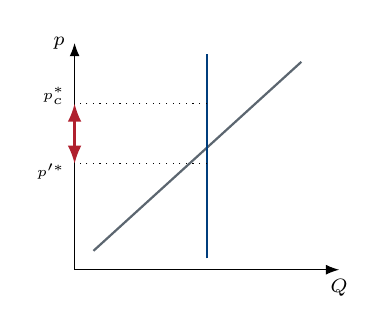
\begin{tikzpicture}[scale=0.48]
        \draw[-{Latex}] (0,0) -- (7,0) node[below, font=\scriptsize]{$Q$};
        \draw[-{Latex}] (0,0) -- (0,6) node[left, font=\scriptsize]{$p$};
        \draw[wugray, thick] (0.5,0.5) -- (6,5.5);
        \draw[wublue, thick] (3.5,0.3) -- (3.5,5.7);
        \draw[dotted] (3.5,4.4) -- (0,4.4);
        \draw[dotted] (3.5,2.8) -- (0,2.8);
        \draw[wured, thick, {Latex}-{Latex}] (0,2.8) -- (0,4.4);
        \node[left, font=\tiny] at (0,4.6) {$p_c^*$};
        \node[left, font=\tiny] at (0,2.6) {$p'^*$};
      \end{tikzpicture}\\[0.3em]
      Quantity can't change --- consumers bear \textbf{100\%} of the burden.
    \end{column}
    \begin{column}{0.5\textwidth}
      \centering \textbf{Perfectly elastic demand}\\[0.2em]
      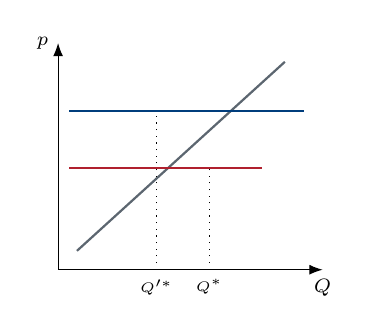
\begin{tikzpicture}[scale=0.48]
        \draw[-{Latex}] (0,0) -- (7,0) node[below, font=\scriptsize]{$Q$};
        \draw[-{Latex}] (0,0) -- (0,6) node[left, font=\scriptsize]{$p$};
        \draw[wugray, thick] (0.5,0.5) -- (6,5.5);
        \draw[wublue, thick] (0.3,4.2) -- (6.5,4.2);
        \draw[wured, thick] (0.3,2.7) -- (5.4,2.7);
        \draw[dotted] (2.6,0) -- (2.6,4.2);
        \draw[dotted] (4,0) -- (4,2.7);
        \node[below, font=\tiny] at (2.6,0) {$Q'^*$};
        \node[below, font=\tiny] at (4,0) {$Q^*$};
      \end{tikzpicture}\\[0.3em]
      Consumer price can't change --- producers bear \textbf{100\%} of the burden.
    \end{column}
  \end{columns}
  \vspace{0.4em}

  \alert{The side of the market with the \emph{less elastic} response bears more of the tax --- regardless of who writes the check.}
\end{frame}

\begin{frame}{Elasticity Determines Incidence}
  \begin{itemize}
    \item In theory, incidence does \emph{not} depend on who is statutorily required to pay --- a tax on sellers and an equivalent tax on buyers have the same economic incidence.
    \item What matters is the \textbf{relative elasticity of supply and demand}:
  \end{itemize}
  \[
    \varepsilon_D = \frac{p_c}{D}\frac{dD}{dp_c}, \qquad \varepsilon_S = \frac{p}{S}\frac{dS}{dp}
  \]
  \vspace{0.3em}
  \begin{alertblock}{Application: excise taxes in Austria}
    Austria taxes tobacco, alcohol, mineral oil, and (since 2022) CO\textsubscript{2} emissions via excise duties. Demand for cigarettes and heating fuel is famously \textbf{inelastic} in the short run --- so standard incidence theory predicts these taxes fall mostly on \emph{consumers}, not producers.
  \end{alertblock}
\end{frame}

\begin{frame}{The Cost of Taxation: Deadweight Loss}
  \begin{block}{Deadweight loss (DWL)}
    The loss in total surplus caused by a tax, \emph{over and above} the revenue it raises --- also called the \textbf{excess burden} of taxation.
  \end{block}
  \vspace{0.3em}
  \begin{itemize}
    \item A tax drives a wedge between the price buyers pay and the price sellers receive. Some trades that were worth doing before the tax are no longer worth doing.
    \item Those forgone trades are the source of DWL: surplus that simply \emph{vanishes} --- it goes to neither the government, consumers, nor producers.
  \end{itemize}
  \srcnote{Gruber, \emph{Public Finance and Public Policy}, Ch.\,19 (The Efficiency Costs of Taxation).}
\end{frame}

\begin{frame}{Visualizing Deadweight Loss}
  \begin{center}
    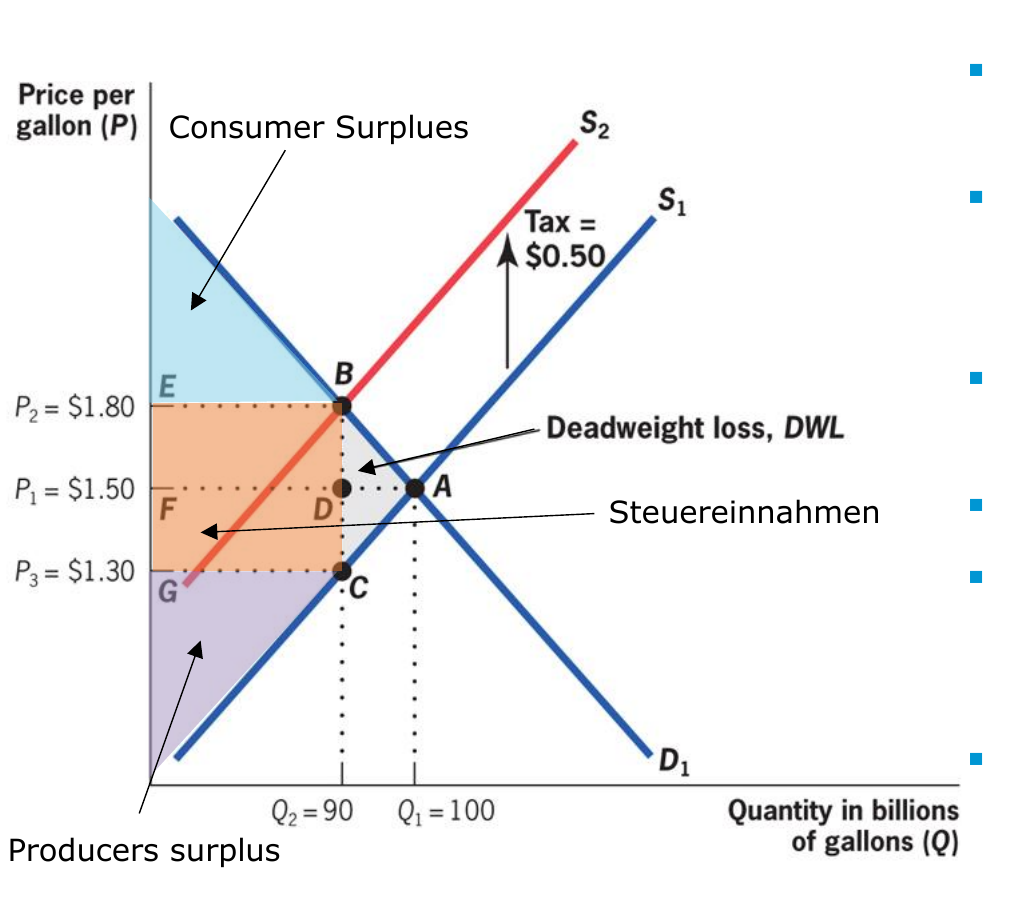
\includegraphics[height=5.3cm]{figures/edu_dwl_diagram.png}
  \end{center}
  \footnotesize
  The tax wedges the price consumers pay ($P_2$) apart from the price producers receive ($P_3$). Quantity falls from $Q_1$ to $Q_2$. The shaded rectangle is tax revenue --- transferred, not lost. The shaded \emph{triangle} is DWL: surplus from trades between $Q_2$ and $Q_1$ that the tax has simply eliminated.
\end{frame}

\begin{frame}{DWL and the Elasticity of Supply and Demand}
  \begin{center}
    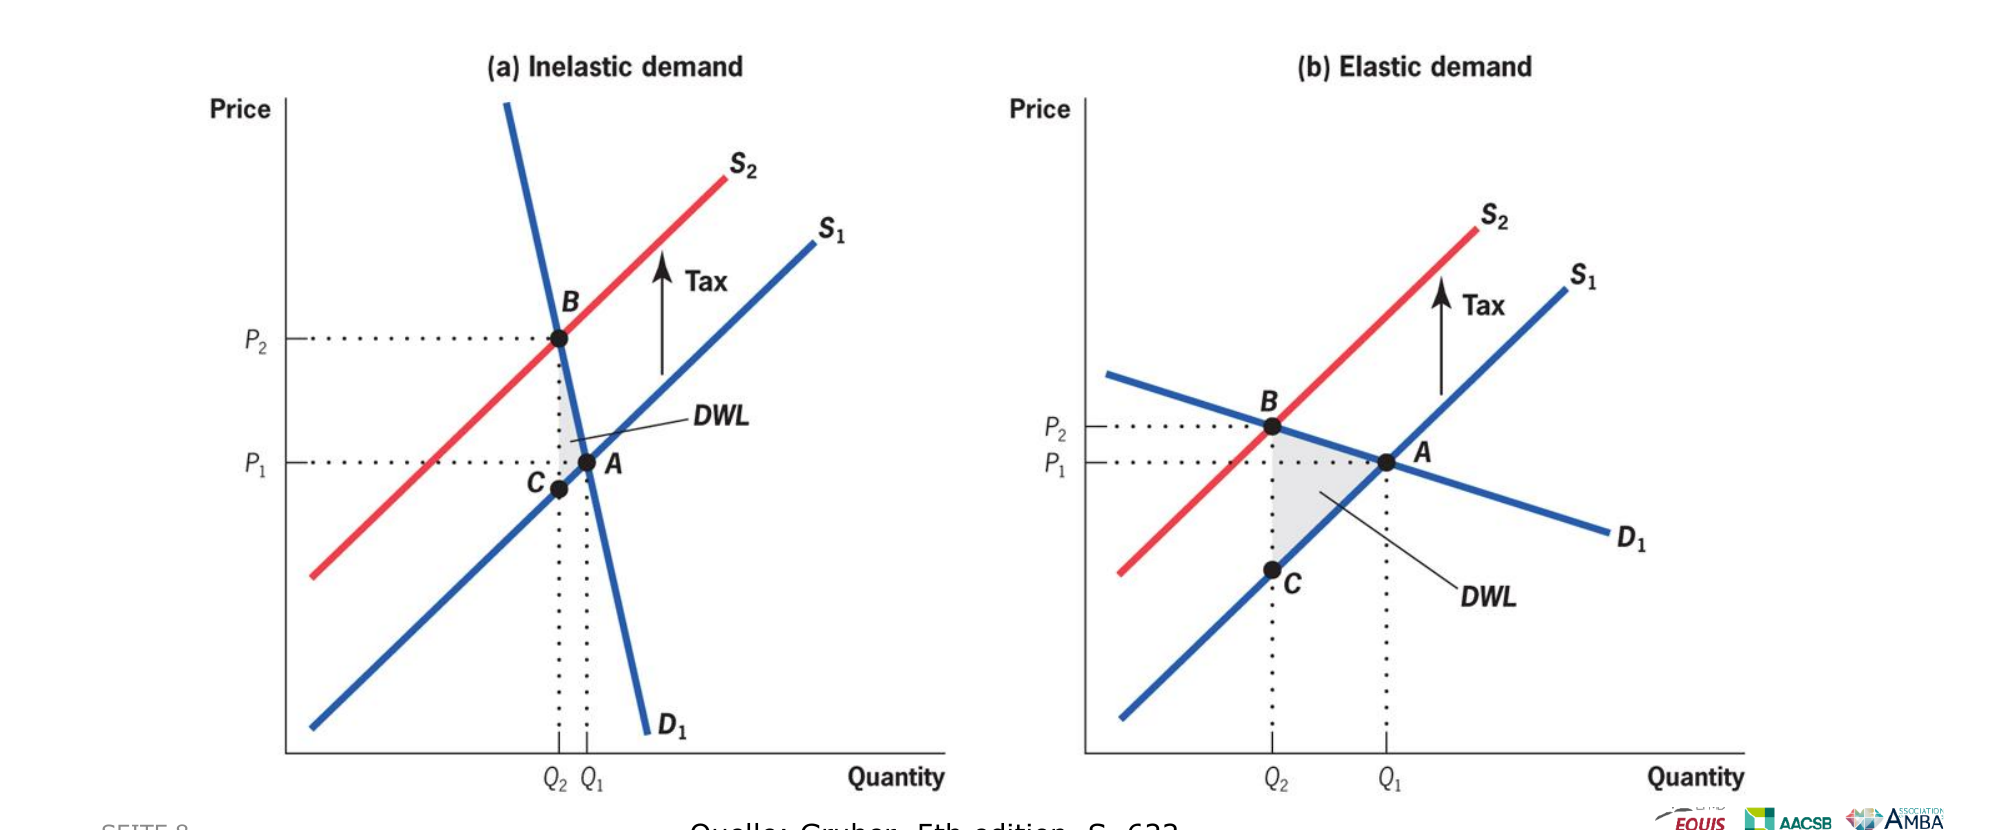
\includegraphics[width=0.92\textwidth]{figures/edu_dwl_elasticity.png}
  \end{center}
  \footnotesize
  The \emph{same-sized} tax produces far less deadweight loss when demand is inelastic (a) than when it is elastic (b): inelastic responses mean fewer valuable trades are given up.\\
  \srcnote{Gruber, 5th ed., p.\,622.}
\end{frame}

\begin{frame}{DWL Rises with the \emph{Square} of the Tax Rate}
  \begin{columns}[T]
    \begin{column}{0.5\textwidth}
      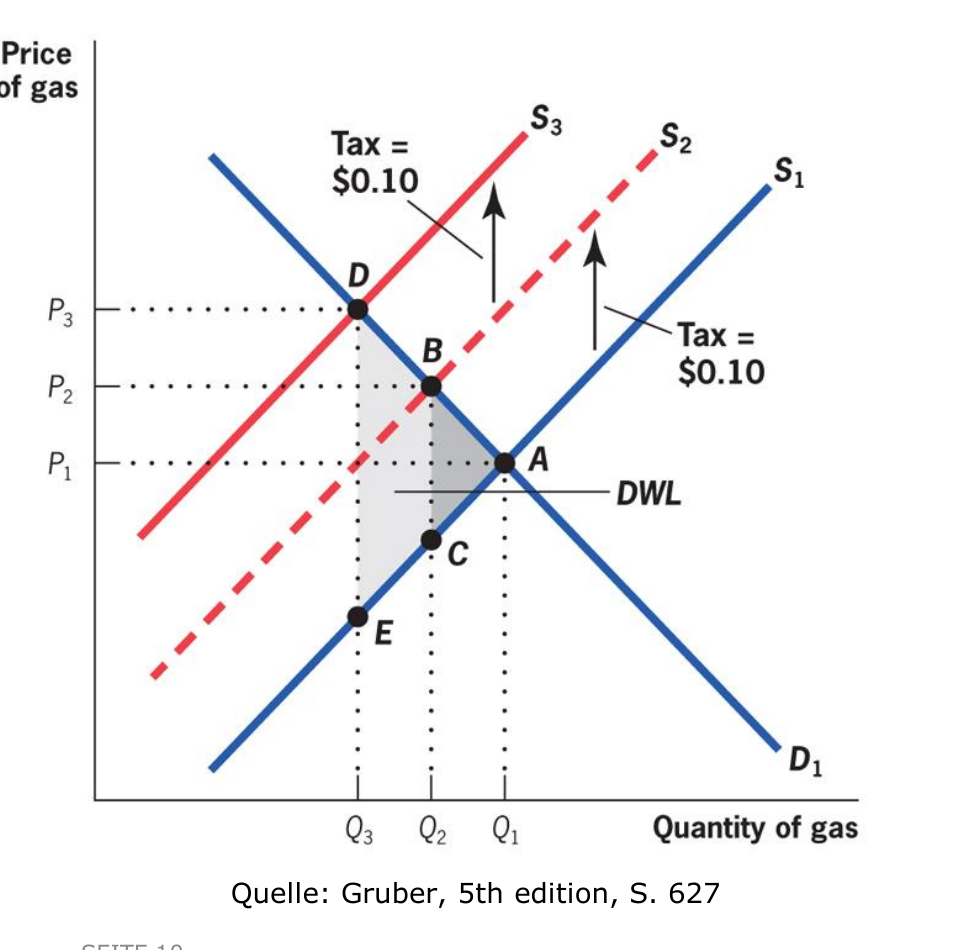
\includegraphics[height=5.5cm]{figures/edu_dwl_convexity.png}
    \end{column}
    \begin{column}{0.5\textwidth}
      \footnotesize
      \begin{itemize}
        \item Doubling a tax roughly \textbf{quadruples} its deadweight loss --- DWL is \emph{convex} in the tax rate.
        \item \textbf{Implication:} to raise a given amount of revenue at minimum efficiency cost, spread taxation thinly across \emph{many} goods rather than taxing one good heavily.
      \end{itemize}
      \vspace{0.3em}
      \srcnote{Gruber, 5th ed., p.\,627.}
    \end{column}
  \end{columns}
\end{frame}

\begin{frame}{Historical Evidence: The Window Tax}
  \begin{center}
    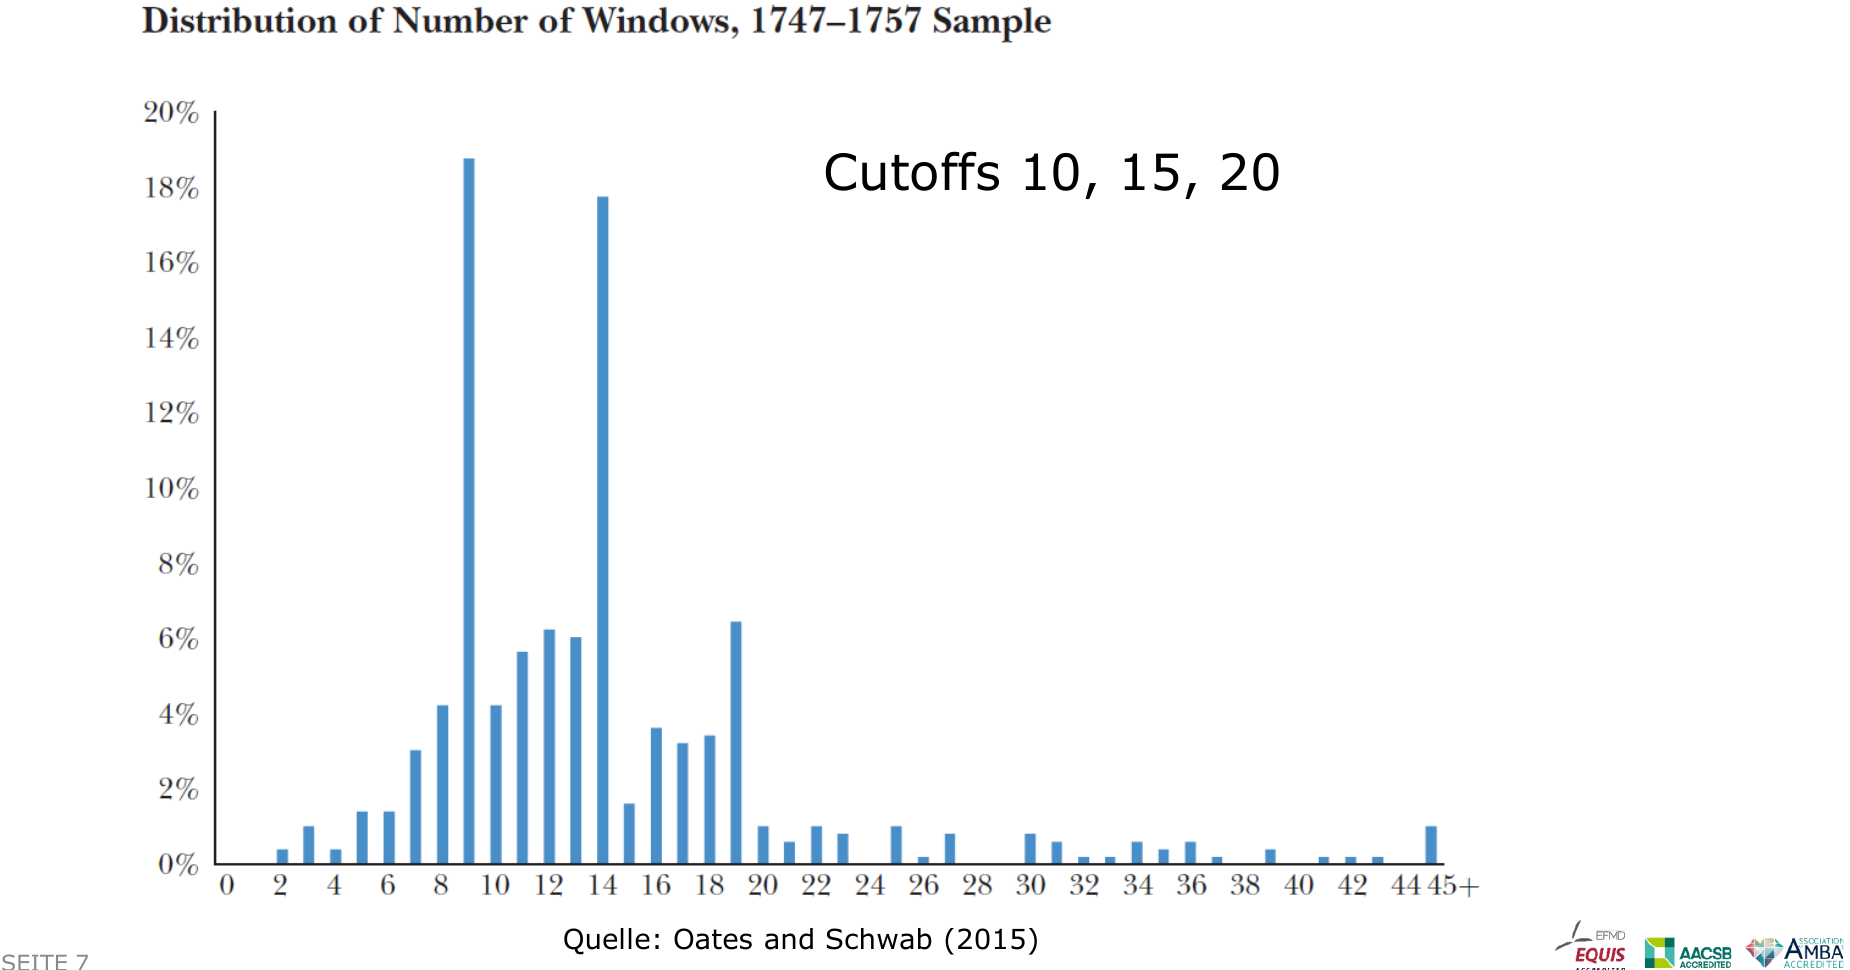
\includegraphics[width=0.68\textwidth]{figures/edu_window_tax_bunching.png}
  \end{center}
  \footnotesize
  England, 1696--1851: homes were taxed on the number of windows above a threshold. Households \textbf{bunched} just below the cutoffs (10, 15, 20) --- literally bricking up windows to dodge the next band. A vivid, visible illustration of the behavioral response that generates deadweight loss.\\
  \srcnote{Oates \& Schwab (2015).}
\end{frame}

\begin{frame}{Taxation Under Monopoly}
  \begin{columns}[T]
    \begin{column}{0.55\textwidth}
      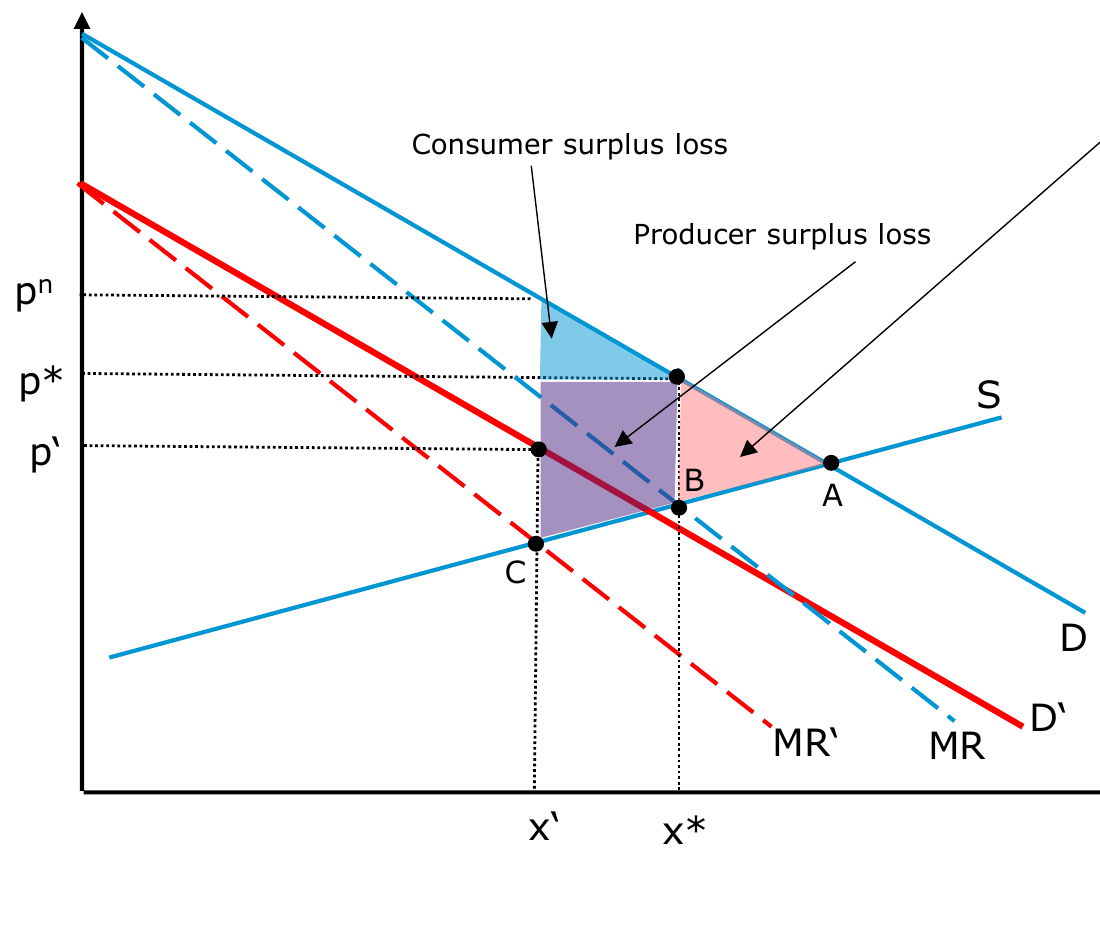
\includegraphics[height=5.0cm]{figures/edu_monopoly_dwl.png}
    \end{column}
    \begin{column}{0.45\textwidth}
      \footnotesize
      \begin{itemize}
        \item A monopolist \emph{already} restricts output below the competitive level, creating its own DWL triangle.
        \item Layering a tax on top shifts $MR$ further, shrinking output again from $x^*$ to $x'$ --- a \emph{second} wedge of consumer and producer surplus loss stacked on the first.
      \end{itemize}
    \end{column}
  \end{columns}
\end{frame}

\begin{frame}{Who Actually Bears Payroll Taxes? The Evidence}
  \begin{center}
    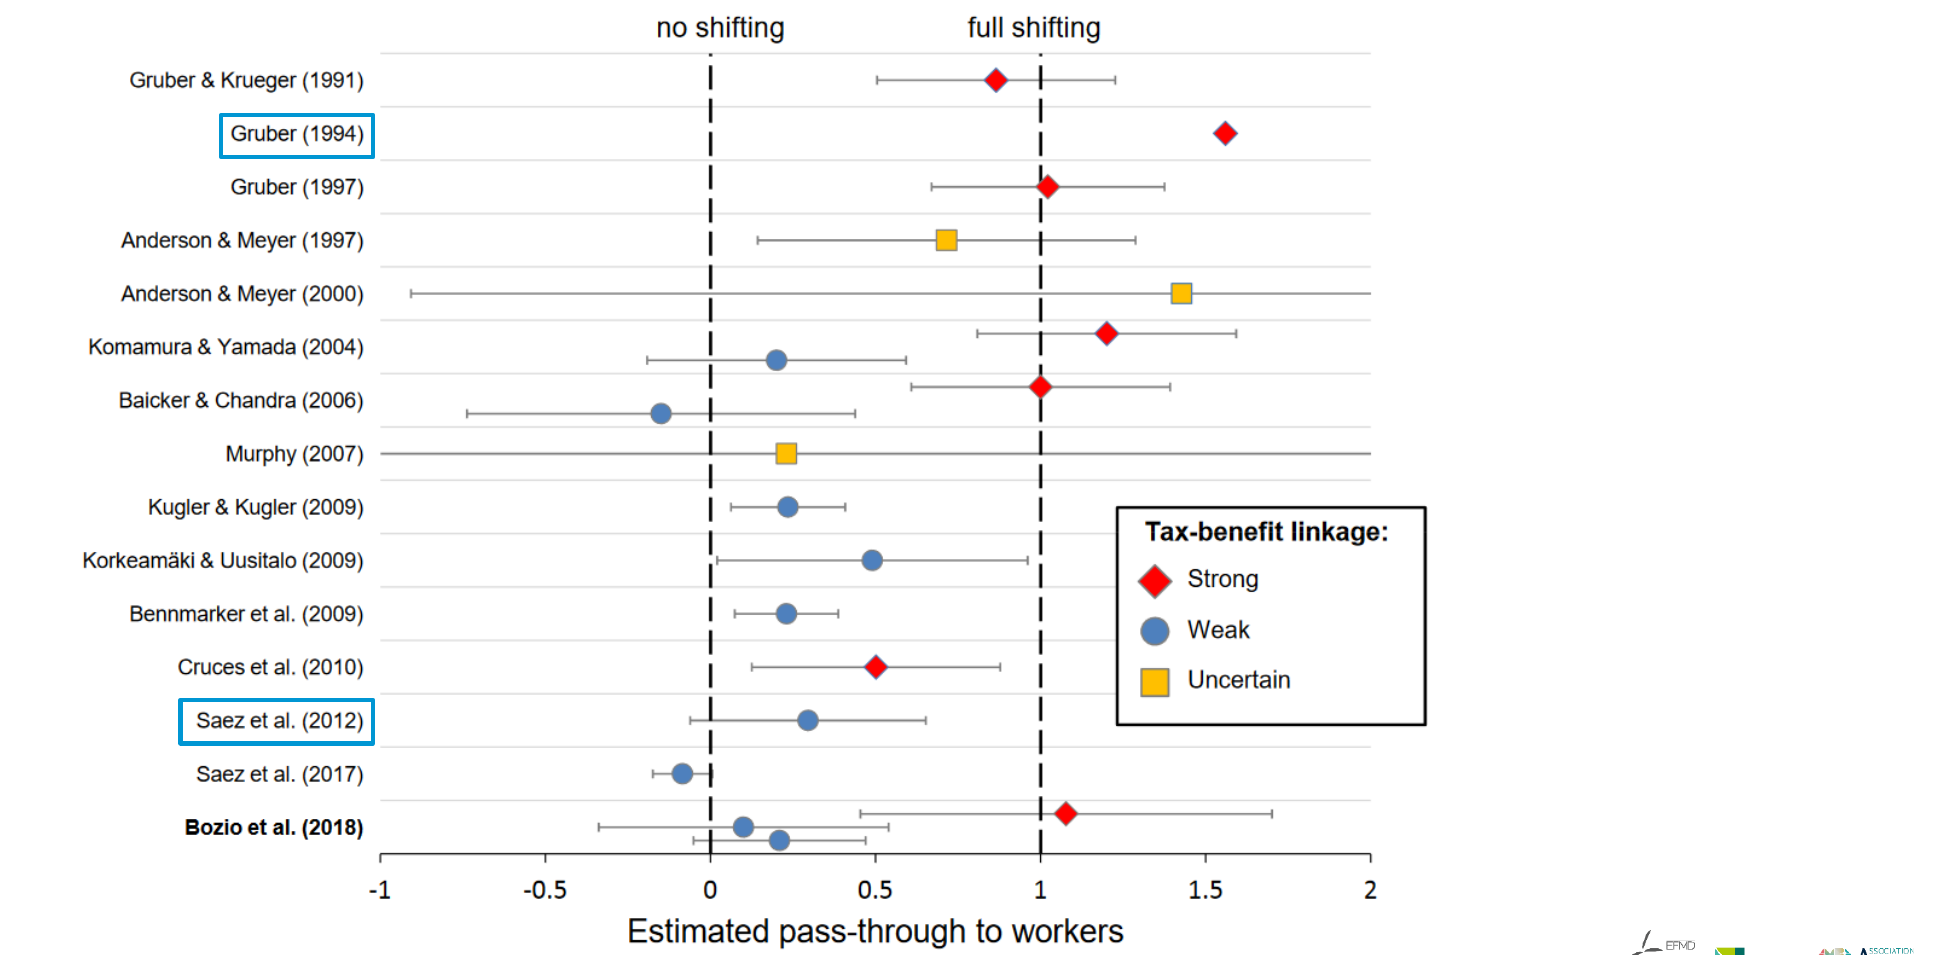
\includegraphics[height=5.6cm]{figures/edu_incidence_forest_plot.png}
  \end{center}
  \footnotesize
  Fifteen quasi-experimental studies estimate how much of a payroll-tax change passes through to workers' wages. Estimates span the full range from 0\% to full shifting --- and tend to be \textbf{higher} when the tax buys a benefit workers clearly value (\emph{strong} tax-benefit linkage, red diamonds) than when the link is weak or absent.
\end{frame}

\begin{frame}{The Equity--Efficiency Trade-off, Revisited}
  \small
  A progressive income tax has two effects:
  \begin{enumerate}
    \item \textbf{Equity gain}: reduces income inequality.
    \item \textbf{Efficiency loss}: people may work less when income is taxed --- if they care about \emph{net}, not gross, pay.
  \end{enumerate}
  \vspace{0.3em}
  The size of the efficiency loss is governed by the \textbf{elasticity of labor supply} (Lecture 2). Governments can dampen it by using tax revenue to subsidize goods complementary to working, such as child care.
  \vspace{0.3em}

  \(\Rightarrow\) ``How Can Scandinavians Tax So Much?'' (Kleven, 2014) --- high-tax Nordic countries also invest heavily in making work easy (child care, low-distortion consumption taxes), which is part of how they sustain such high tax revenue with limited efficiency loss.\\
  \srcnote{Kleven, H., \emph{Journal of Economic Perspectives} 28(4), 2014, cited in Leenders, Part IV.}
\end{frame}

% =============================================================
\section{4.3 Measuring the Fairness of Tax Systems}

\begin{frame}{Average vs.\ Marginal Tax Rates}
  \begin{block}{Marginal tax rate}
    The share of the \emph{next euro} of taxable income paid in tax.
  \end{block}
  \begin{block}{Average tax rate}
    Total tax paid, divided by total (gross) income --- a weighted average of all the marginal rates paid along the way.
  \end{block}
\end{frame}

\begin{frame}{Austria's 2026 Income Tax Brackets}
 \begin{table}
 	\centering
 	\begin{tabular}{@{}lr@{}}
 		\toprule
 		\textbf{ } & \textbf{Tax rate} \\
 		\midrule
 		13.539 und darunter & 0\,\% \\
 		über 13.539 bis 21.992 & 20\,\% \\
 		über 21.992 bis 36.458 & 30\,\% \\
 		über 36.458 bis 70.365 & 40\,\% \\
 		über 70.365 bis 104.859 & 48\,\% \\
 		über 104.859 bis 1.000.000 & 50\,\% \\
 		über 1.000.000\textsuperscript{1)} & 55\,\% \\
 		\bottomrule
 	\end{tabular}

 \end{table}


  \vspace{0.5em}
   \small
  The 55\% top bracket is a temporary surcharge. Brackets are progressive: each additional euro is taxed at a higher rate than the last.\\

\end{frame}



\begin{frame}{Worked Example: Lena's Tax Bill}
	\footnotesize
	Lena has taxable income of \texteuro{}80,000. Walking up the bracket schedule:
	\[
	(\text{\texteuro}8{,}453 \times 0.20) + (\text{\texteuro}14{,}466 \times 0.30) + (\text{\texteuro}33{,}907 \times 0.40) + (\text{\texteuro}9{,}635 \times 0.48) = \text{\texteuro}24{,}218.00
	\]
	Her disposable income: 80,000-24,218=55,782
	\vspace{0.3em}
	\begin{itemize}
		\item Lena's \textbf{marginal} tax rate is \textbf{48\%} --- the rate on her next euro earned.
		\item Lena's \textbf{average} tax rate is \(\text{\texteuro}24{,}218.00 / \text{\texteuro}80{,}000 = \mathbf{30.3\%}\).
	\end{itemize}
	\vspace{0.3em}

	The gap between the two --- 48\% vs.\ 30.3\% --- is entirely due to progressivity: the first \texteuro{}13,539 was tax-free, and every bracket below her marginal one was taxed at a lower rate.
\end{frame}

\begin{frame}{Vertical and Horizontal Equity}
  \begin{block}{Vertical equity}
    Groups with more resources should pay higher taxes than groups with fewer resources.
  \end{block}
  \begin{block}{Horizontal equity}
    Individuals who are similar, but make different choices, should be treated the same by the tax system.
  \end{block}
  \vspace{0.3em}
  \begin{itemize}
    \item A \textbf{progressive} system: average tax rates \emph{rise} with income.
    \item A \textbf{proportional} (flat) system: average tax rates are \emph{constant}.
    \item A \textbf{regressive} system: average tax rates \emph{fall} with income.
  \end{itemize}
\end{frame}

\begin{frame}{When ``Fair'' Causes a Riot}
  \small
  In March 1990, rioters in London set fire to parked cars and smashed storefronts, injuring more than 400 people. The cause: Margaret Thatcher's proposal to replace property taxes with a \textbf{poll tax} --- a flat charge levied \emph{equally} on every adult, rich or poor.
  \vspace{0.3em}
  \begin{alertblock}{Why it provoked outrage}
    The tax burden shifted away from wealthy property owners and onto poorer citizens who hadn't previously paid property tax at all --- a textbook violation of \textbf{vertical equity}. Thatcher was ousted as Conservative leader soon after; the tax was abandoned.
  \end{alertblock}
  \vspace{0.3em}

  (England's last attempt at such a tax, in 1381, ended with the beheading of several prominent officials.)\\

\end{frame}

\begin{frame}{Austria's Own Fairness Debate: \emph{Kalte Progression}}
  \footnotesize
  \begin{block}{The problem}
    With fixed, progressive brackets, \textbf{inflation} pushes people into higher brackets even when their \emph{real} income hasn't grown --- a stealth tax increase known as \emph{kalte Progression} (bracket creep).
  \end{block}
  \vspace{0.3em}
  \begin{itemize}
    \item Effective 1 January 2023, Austria began \textbf{automatically indexing} tax brackets to inflation: two-thirds of the inflation adjustment happens automatically by law each year; the remaining third is allocated at the government's discretion via a separate ``\emph{Progressionsabgeltungsgesetz}.''
    \item The top \texteuro{}1{,}000{,}000 / 55\% bracket is \emph{excluded} from indexation.
  \end{itemize}


 \end{frame}

% =============================================================
\section{Effective Tax Rates, Transfers, and Work Incentives}

\begin{frame}{Beyond the Bracket: Effective Marginal Tax Rates}
  \begin{block}{Effective marginal tax rate (EMTR)}
    The share of an \emph{extra euro} of earnings lost to \textbf{taxes and withdrawn benefits} combined --- not just the statutory income-tax bracket.
  \end{block}
  \vspace{0.3em}
  \begin{itemize}
    \item Means-tested transfers (housing benefit, childcare subsidies, unemployment benefits) phase \emph{out} as earnings rise --- each euro of phase-out is economically identical to a euro of tax.
    \item A worker's true disincentive to earn more can be far higher than their income-tax bracket suggests once benefit withdrawal is added in.
  \end{itemize}
  \srcnote{Gruber, \emph{Public Finance and Public Policy}, Ch.\,21 (Taxation of Labor Income).}
\end{frame}

\begin{frame}{Top Effective Marginal Rates Across Europe}
  \begin{center}
    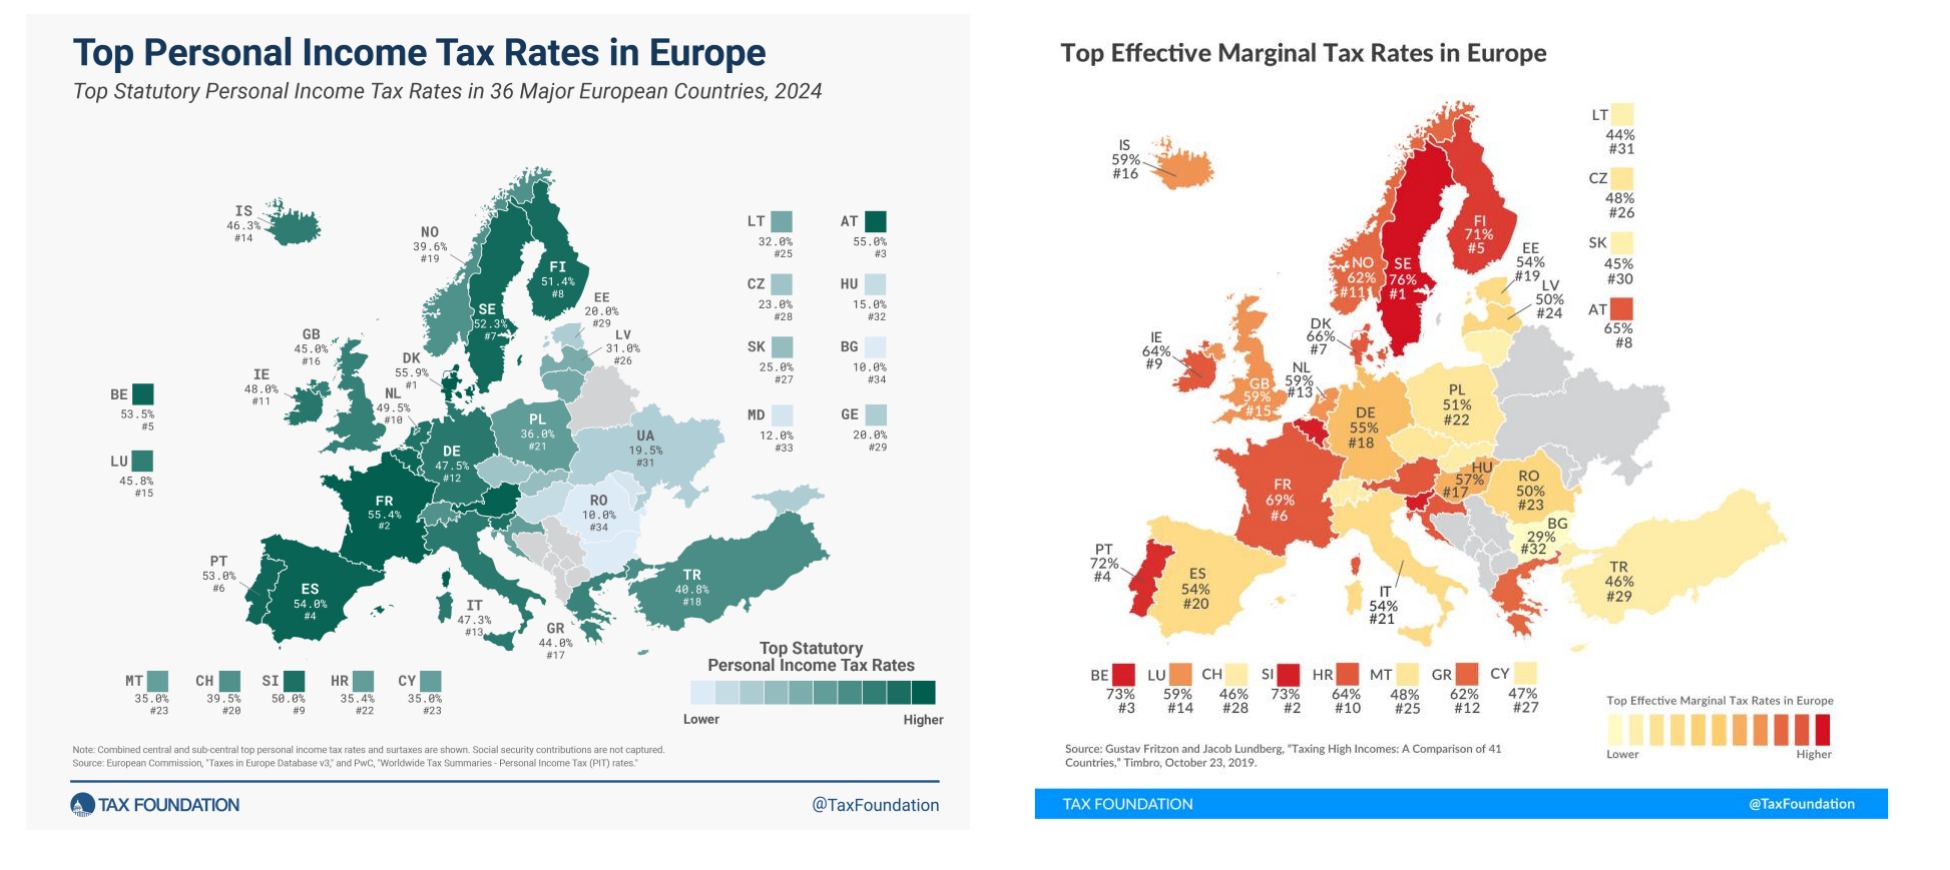
\includegraphics[width=0.85\textwidth]{figures/edu_effective_marginal_rate_maps.png}
  \end{center}
  \footnotesize
  Statutory top rates (left) and top \emph{effective} marginal rates once benefit phase-outs and social contributions are added (right) can rank countries very differently. Austria: \#3 by statutory top rate (55\%), \#8 by effective marginal rate (65\%).
\end{frame}

\begin{frame}{The Participation Tax Rate}
  \begin{block}{Participation tax rate}
    The share of gross earnings lost to taxes \emph{and} forgone benefits when moving from \textbf{not working at all} to working --- the ``is it worth taking a job'' rate, as distinct from the EMTR (``is it worth earning one more euro'').
  \end{block}
  \vspace{0.3em}
  A high participation tax rate is exactly the ``benefit cliff'' or ``welfare trap'' problem: means-tested systems can leave people with almost no net gain from entering the labor force at all.
\end{frame}

\begin{frame}{The Tax-Rate Benefit Cliff: US vs.\ France}
  \begin{center}
    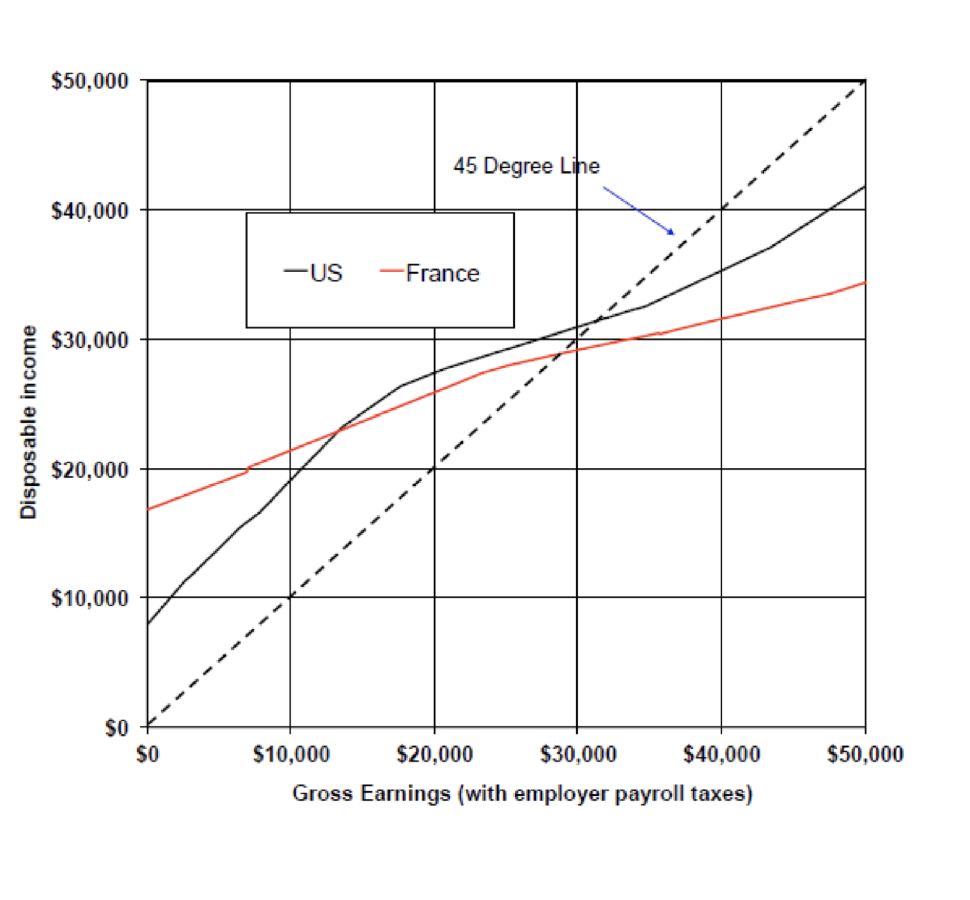
\includegraphics[height=5.1cm]{figures/edu_benefit_cliff_us_france.png}
  \end{center}
  \footnotesize
  Disposable income against gross earnings (incl.\ employer payroll tax), US vs.\ France. Where the curve runs \emph{flatter} than the 45\textdegree{} line, an extra euro of gross earnings buys less than a euro of disposable income --- the US delivers a bigger gain from entering work at all, while France imposes the higher \emph{marginal} burden in the middle of the distribution.\\
  \srcnote{Piketty \& Saez (2012).}
\end{frame}

\begin{frame}{Designing a Better Phase-Out: The EITC}
  \begin{center}
    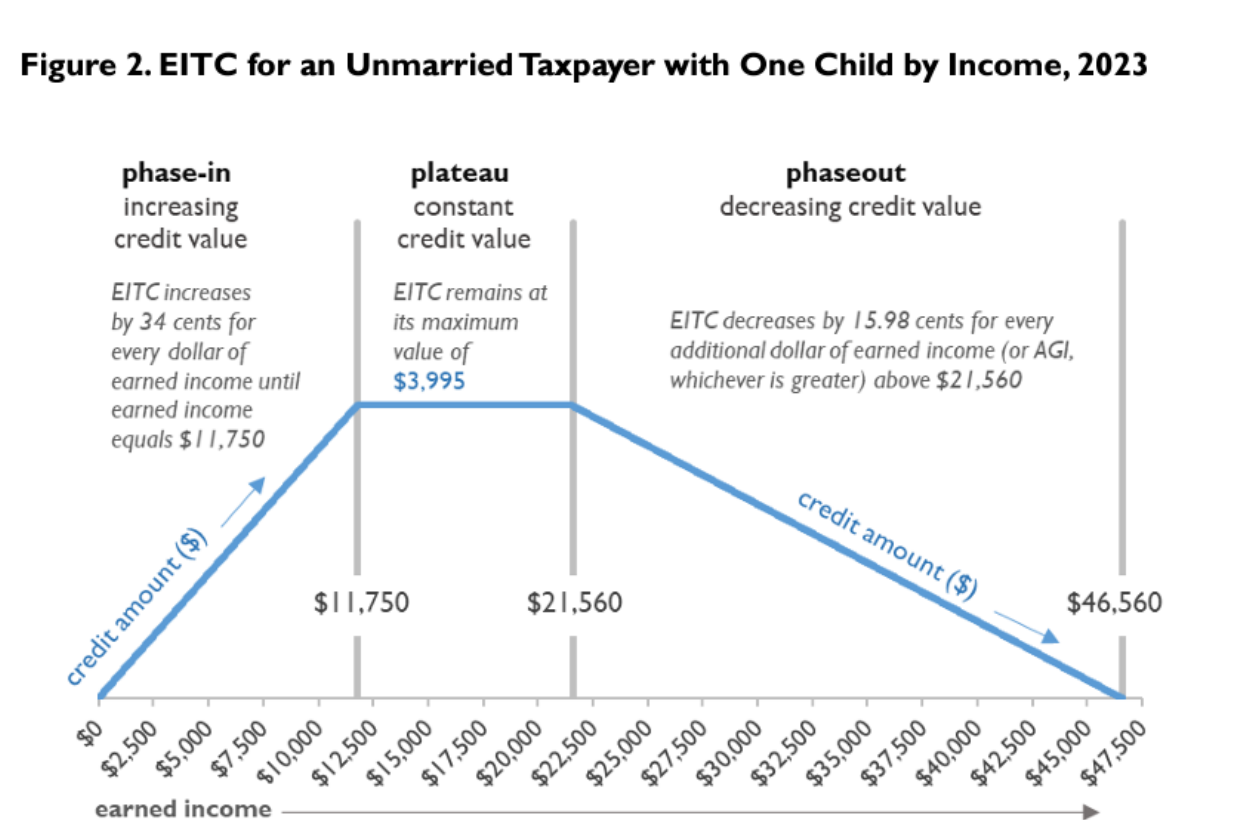
\includegraphics[height=5.2cm]{figures/edu_eitc_schedule.png}
  \end{center}
  \footnotesize
  The US Earned Income Tax Credit is deliberately \textbf{hump-shaped}: it \emph{subsidizes} the first euros earned (phase-in), so entering the labor force always pays --- solving the participation problem --- then phases out gradually, still leaving a (smaller) EMTR problem in the phase-out range.
\end{frame}

\begin{frame}{UBI vs.\ Means-Tested Transfers: An Equivalence}
  \small
  \begin{itemize}
    \item A \textbf{universal basic income} (UBI) financed by a flat tax on all earnings, and a \textbf{means-tested transfer} that phases out with earnings, can be made mathematically \emph{identical} in their net effect on any given household's budget constraint.
    \item The real policy choice is not ``universal vs.\ targeted transfer'' in the abstract --- it is about \emph{where} the phase-out happens, how steep it is, and the \textbf{administrative/stigma costs} of means-testing versus the \textbf{fiscal cost} of paying transfers to people who don't need them.
  \end{itemize}
  \vspace{0.3em}
  \alert{Discussion:} which trade-off would you take for Austria's \emph{Sozialhilfe}/\emph{Arbeitslosengeld} system?
\end{frame}

\begin{frame}{Do Benefit Levels Actually Change Behavior? Evidence from UI}
  \footnotesize
  \begin{itemize}
    \item Standard theory: more generous unemployment insurance (UI) should \emph{lengthen} unemployment spells, since it raises the reservation wage and lowers the cost of continued search.
    \item Natural experiments exploiting discontinuities in UI generosity (benefit level, potential duration) across US states and European countries consistently find this effect --- but it is \textbf{modest} in size, and much of the ``spike'' in job-finding just before benefits expire reflects \emph{timing} of job offers already in hand, not new search effort.
  \end{itemize}
  \vspace{0.3em}
  \centering
  The size of this moral-hazard effect is exactly the elasticity that determines the equity--efficiency trade-off (this lecture) for any transfer program.
\end{frame}

% =============================================================
\section{4.4 Defining the Income Tax Base}

\begin{frame}{The Haig-Simons Comprehensive Income Definition}
  \begin{block}{Haig-Simons income}
    Taxable resources = an individual's \emph{ability to pay} = total consumption during the year \(+\) any increase in wealth.
  \end{block}
  \vspace{0.3em}
  \begin{itemize}
    \item In principle, comprehensive income improves \emph{both} vertical equity (all resources are taxed, however received) \emph{and} horizontal equity (the form compensation takes shouldn't matter).
    \item In practice, every real tax system deviates from this ideal --- the question is whether each deviation is justified.
  \end{itemize}
  \srcnote{Gruber, \emph{Public Finance and Public Policy}, \S18.4.}
\end{frame}

\begin{frame}{Austria vs.\ the US: In-Kind Compensation}
  \begin{itemize}
    \item The classic Haig-Simons violation in th US: employer-provided \textbf{health insurance} is not taxed as income, even though it clearly raises a worker's ability to consume.
    \item Austria takes a stricter approach for many in-kind benefits: the \emph{Sachbezugswerteverordnung} taxes the value of a company car, subsidized housing, and other in-kind perks as part of wage income.
  \end{itemize}


\end{frame}

\begin{frame}{Deviations for Ability-to-Pay and Earning Costs}
  \small
  \begin{itemize}
    \item \textbf{Ability-to-pay deviations}: Austria's \emph{außergewöhnliche Belastungen} (extraordinary burden deductions) let taxpayers deduct large, involuntary costs --- medical expenses, disaster losses --- on the same logic as Gruber's ``fire damage'' example: these expenditures aren't really \emph{consumption}, so they shouldn't count as ability to pay.
    \item \textbf{Cost-of-earning-income deviations}: Austria's \emph{Werbungskosten} let workers deduct job-related expenses, including the \emph{Pendlerpauschale} (commuter allowance, Lecture 1) --- the same logic as deducting business costs from Haig-Simons income.
  \end{itemize}
  \vspace{0.3em}
  \centering
  Both are easy to justify in principle --- and hard to draw a clean line around in practice (was that lunch a business cost, or consumption?).
\end{frame}

\begin{frame}{Housing}
  \footnotesize
  \begin{itemize}
    \item Whether you rent or own, you consume \texteuro{}X/month of housing services --- your \emph{imputed rental value}. A true Haig-Simons tax would treat renters and owners identically.
    \item The \textbf{US} does not tax imputed rental income, \emph{but} lets owners deduct mortgage interest --- a large, one-sided subsidy to owning (\(\approx\)\texteuro{}80bn/year in forgone US federal revenue)
    \item Empirical research finds little evidence that home ownership has positive social benefits

    Austria   taxes owners and renters rather symmetrically

  \end{itemize}
\end{frame}

\begin{frame}{Deductions vs.\ Credits}
  \begin{block}{Tax deduction}
    Reduces \emph{taxable income} --- its value to the taxpayer is \(\$(1-t)\) per euro, so it's worth \emph{more} to people in higher brackets.
  \end{block}
  \begin{block}{Tax credit}
    Reduces \emph{tax owed} directly --- worth the same to everyone, regardless of bracket, and thus more progressive.
  \end{block}
  \vspace{0.3em}

  A \textbf{refundable} credit goes further still: it pays out even to people who owe little or no tax --- turning the tax system into a delivery mechanism for cash transfers to low earners.
\end{frame}

\begin{frame}{Austria's Own Refundability Debate: \emph{Familienbonus Plus}}
  \footnotesize
  Introduced in 2019 as a tax \textbf{credit} (not a deduction) for families with children.
  \begin{itemize}
    \item 2024 value: \texteuro{}2{,}000.16/year per child under 18; \texteuro{}700.08/year per child 18 or older.
    \item Because it's a credit against tax owed, it delivers \emph{nothing} to a parent who owes little or no income tax --- exactly the refundability problem the US Child Tax Credit debate raises.
    \item Austria's partial fix: the \emph{Kindermehrbetrag} (2024: \texteuro{}700/child) tops up low earners who claim the sole-earner/single-parent credit, closing the gap between their (near-zero) tax liability and \texteuro{}700.
  \end{itemize}
  \vspace{0.3em}
  \centering
  \alert{Discussion:} does the Kindermehrbetrag fully solve the vertical-equity problem of a non-refundable credit, or only partly?\\
  \srcnote{Bundeskanzleramt; BMF, Familienbonus Plus \& Kindermehrbetrag (2024).}
\end{frame}

\begin{frame}{Tax Expenditures}
  \begin{block}{Tax expenditures}
    Revenue the government forgoes through special exclusions, deductions, credits, or preferential rates --- functionally equivalent to direct spending, just routed through the tax code instead of the budget.
  \end{block}
  \vspace{0.3em}
  \centering
  In the US, tax expenditures total over \texteuro{}1 trillion/year --- more than 40\% of total tax revenue. Every deduction and credit on the last several slides (Familienbonus Plus, Werbungskosten, außergewöhnliche Belastungen) is, by this definition, an Austrian tax expenditure too.\\
  \srcnote{Gruber, \emph{Public Finance and Public Policy}, \S18.5, citing U.S.\ Department of the Treasury (2021a).}
\end{frame}

% =============================================================
\section{The Rise of the Fiscal State}

\begin{frame}{How Did We Get Progressive Taxation?}
  \small
  \begin{itemize}
    \item Top marginal income-tax rates were in the single digits almost everywhere before 1900 --- then rose sharply, above all in the US, UK, Sweden, Germany, and France, from the 1910s onward.
    \item \textbf{World War I} acted as the catalyst: many countries raised top rates on income and inheritances explicitly as a ``conscription of capital'' to match the conscription of soldiers.
    \item The wartime rate hikes only \emph{stuck} because of lasting technological and institutional changes: employer-based withholding, and --- eventually --- the end of bank secrecy.
  \end{itemize}
  \vspace{0.3em}
  \begin{alertblock}{Austria's own version of that last point}
    Austria was long known for strict \emph{Bankgeheimnis} (bank secrecy). That changed with the OECD's Common Reporting Standard: Austria began automatically exchanging account data with foreign tax authorities starting September 2017.
  \end{alertblock}
  \srcnote{Leenders, Part IV, citing Piketty, \emph{Capital and Ideology} (2020); Gemeinsamer Meldestandard-Gesetz (GMSG), effective 2016--2017.}
\end{frame}

\begin{frame}{The Long-Run Fall in Top Income Shares: L-Shaped}
  \begin{center}
  %  
\includegraphics[height=4.9cm]{figures/top1pct_europe_japan_lshaped.png}
  \end{center}
  \centering
  \footnotesize
  The rate hikes on the previous slide show up directly in the data: top 1\% income shares in France, Japan, and Sweden collapsed from \(\approx\)18--20\% before WWII to \(\approx\)4--8\% by the 1970s--80s --- and \textbf{stayed low} since.\\
  \srcnote{World Top Incomes Database / WID.world.}
\end{frame}

\begin{frame}{...vs.\ U-Shaped: English-Speaking Countries}
  \begin{center}
   % 
\includegraphics[height=2.85cm]{figures/top1pct_english_speaking_ushaped.png}
  \end{center}
  \footnotesize
  The US, UK, and Canada saw an equally sharp WWII-era collapse --- but then \textbf{rebounded} close to pre-war levels by the 2010s.
  \vspace{0.3em}
  \begin{alertblock}{Why the difference?}
    Piketty, Saez \& Stantcheva (2014) link this directly to \emph{tax} policy: countries that cut top marginal rates the most after 1980 (the US, UK) saw the largest rebound in top income shares; countries that kept rates comparatively high (France, Germany, much of Continental Europe) saw much smaller rebounds.
  \end{alertblock}
  \srcnote{World Top Incomes Database / WID.world; Piketty, Saez \& Stantcheva, ``Optimal Taxation of Top Labor Incomes,'' \emph{AEJ: Economic Policy} 6(1), 2014.}
\end{frame}

\begin{frame}{Why This History Matters}
  \begin{itemize}
    \item The rise in top rates on the wealthy over the twentieth century is a major part of the story behind the dramatic \emph{fall} in income and wealth inequality across the same period (Lecture 1).
    \item Total tax revenue as a share of national income rose alongside it, from roughly 5--10\% (1870) to 30--55\% (today) across today's rich democracies --- with the US consistently at the \emph{low} end of that range and the Nordic countries at the \emph{high} end.
  \end{itemize}
  \vspace{0.3em}
  \centering
  \alert{This isn't ancient history --- it's the direct backdrop to the debates in this lecture: what should be taxed, how progressively, and how the tax base should be defined.}\\
  \srcnote{Leenders, Part IV, citing Piketty (2020) and long-run OECD/WID revenue series.}
\end{frame}

\begin{frame}{How High \emph{Should} Top Rates Be? Optimal Taxation}
  \small
  \begin{itemize}
    \item A purely \textbf{utilitarian} government would want to redistribute from rich to poor until marginal utilities are equalized --- absent any behavioral response, this argues for very high top rates.
    \item But taxes change behavior: push the rate high enough and people work less, avoid, or evade --- so tax \emph{revenue} does not rise one-for-one with the rate.
  \end{itemize}
  \begin{block}{The Laffer curve}
    Tax revenue as a function of the tax rate: it is zero at $t=0\%$ (no tax) \emph{and} at $t=100\%$ (nobody bothers working or reporting income), and reaches a maximum somewhere in between.
  \end{block}
\end{frame}

\begin{frame}{US Top Marginal Rates, 1913--2018}
  \begin{center}
    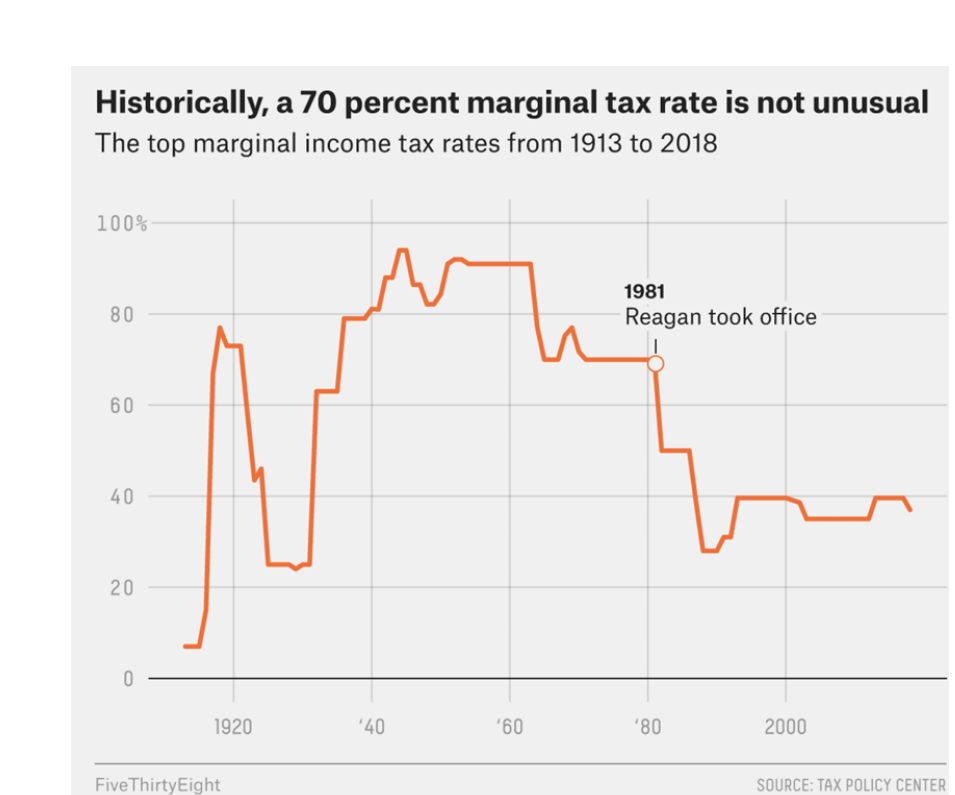
\includegraphics[height=5.3cm]{figures/edu_top_rate_history_us.png}
  \end{center}
  \footnotesize
  A 70\%+ top marginal rate was the American \emph{norm}, not the exception, for nearly 50 years --- reaching over 90\% during WWII and staying above 70\% until the Reagan cuts of 1981.\\
  \srcnote{FiveThirtyEight / Tax Policy Center.}
\end{frame}

\begin{frame}{Top Rates Today: Austria in the European Distribution}
  \begin{center}
    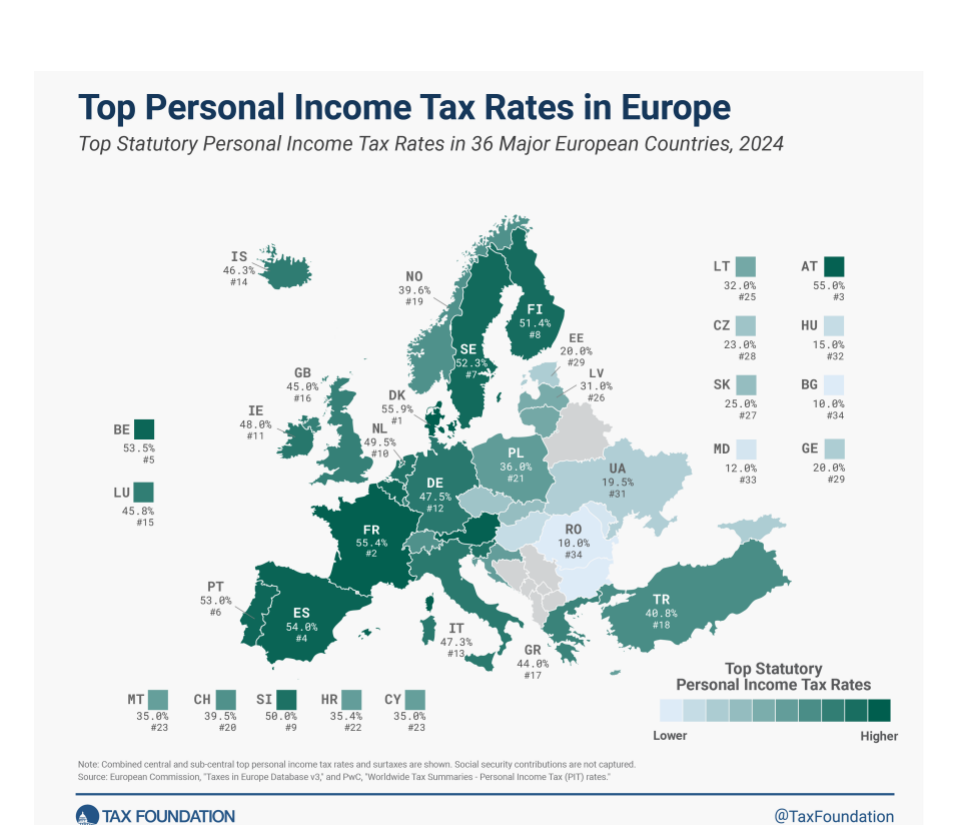
\includegraphics[height=5.3cm]{figures/edu_top_rate_europe_map.png}
  \end{center}
  \footnotesize
  Austria's 55\% top statutory rate ranks \#3 of 36 European countries in 2024 --- behind only Denmark and France.\\
  \srcnote{Tax Foundation; European Commission, Taxes in Europe Database.}
\end{frame}

\begin{frame}{Where Is the Peak of the Laffer Curve?}
  \small
  \begin{itemize}
    \item Its exact location depends entirely on the \textbf{elasticity of taxable income (ETI)}: how much reported income shrinks as the marginal rate rises.
    \item Realistic ETI estimates (\(\approx\)0.2--0.5 for most workers, higher for top earners who have more avoidance margins) put the revenue-maximizing top rate somewhere around 60--80\% --- \emph{well above} most current top rates, but far short of 100\%.
    \item \textbf{Two problems with using this as a policy target:} (i) revenue-maximizing is not the same as \emph{welfare}-maximizing --- a government might rationally choose a lower rate; (ii) reported income can fall through pure \emph{avoidance} (shifting income, timing, relabeling) rather than less real work --- which is a transfer to tax lawyers and accountants, not a genuine efficiency gain from working less.
  \end{itemize}
\end{frame}

\begin{frame}{Bunching Evidence: How Elastic Is Taxable Income, Really?}
  \begin{center}
    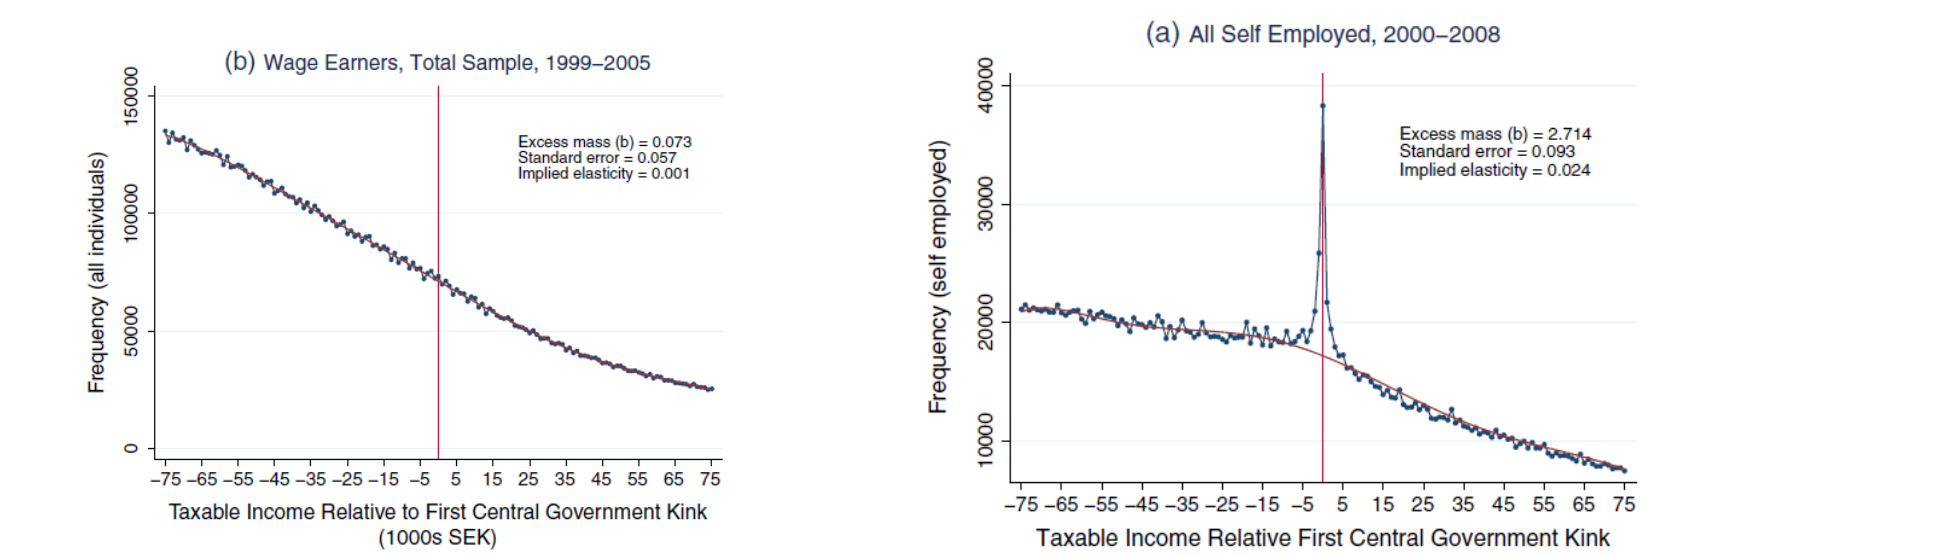
\includegraphics[width=0.85\textwidth]{figures/edu_bunching_sweden.png}
  \end{center}
  \footnotesize
  Sweden: bunching at a central-government tax \textbf{kink} is barely visible for ordinary wage earners (left, implied elasticity 0.001) but sharp for the \textbf{self-employed} (right, implied elasticity 0.024) --- who have far more scope to shift reported income around a threshold.\\
  \srcnote{Bastani \& Selin (2014).}
\end{frame}

\begin{frame}{A Natural Experiment: Switzerland's ``Tax Holiday''}
  \begin{center}
    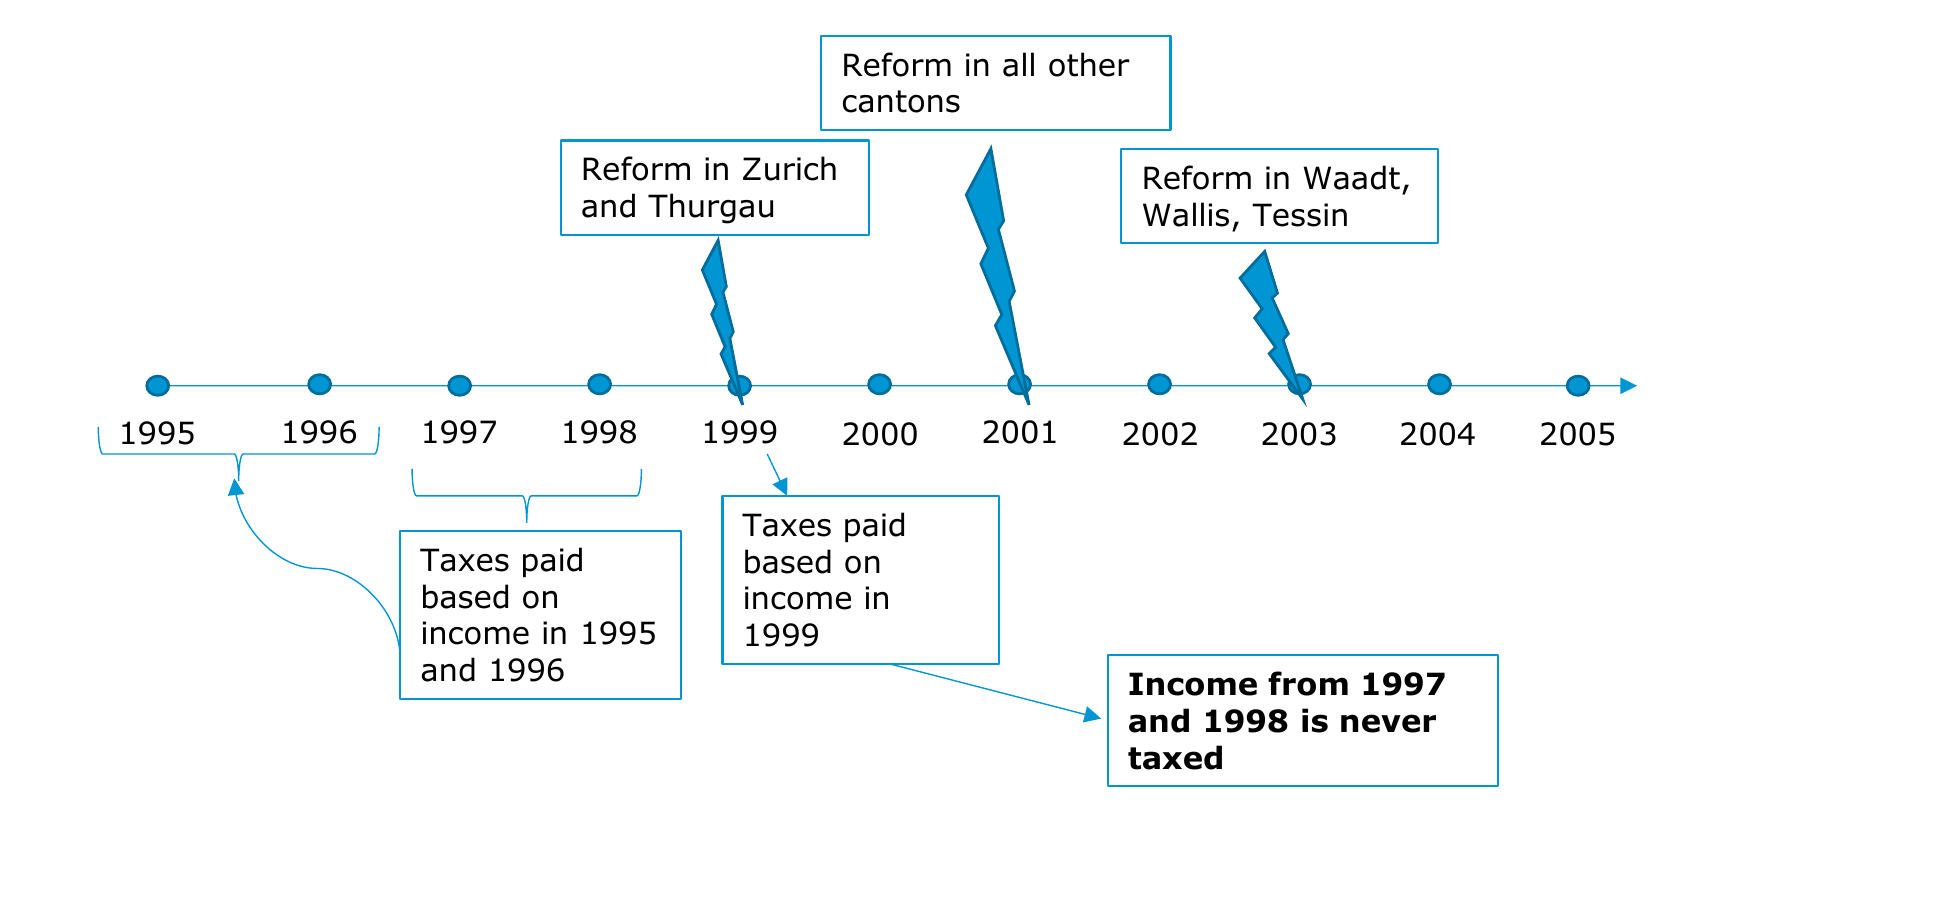
\includegraphics[width=0.72\textwidth]{figures/edu_swiss_tax_holiday.png}
  \end{center}
  \footnotesize
  Swiss cantons switched from taxing the \emph{average} of the previous two years' income to taxing \emph{current-year} income at different dates (1999--2003). Income earned in the untaxed transition years (1997--1998) was never taxed at all --- a one-time, unrepeatable natural experiment in a temporary 100\% marginal-rate cut.
\end{frame}

\begin{frame}{The Formal Labor-Supply Model}
  \footnotesize
  A worker chooses hours $h$ and consumption $c$ to maximize utility $u(c, h)$ subject to the budget constraint
  \[
    c = w(1-t)h + N,
  \]
  where $w$ is the pre-tax wage, $t$ the tax rate, and $N$ non-labor income.
  \vspace{0.3em}
  \begin{itemize}
    \item A tax on labor income lowers the \emph{net} wage $w(1-t)$ --- this has two offsetting effects on hours worked:
    \begin{itemize}
      \item \textbf{Substitution effect}: leisure is now relatively cheaper $\rightarrow$ work \emph{less}.
      \item \textbf{Income effect}: you're poorer at any given hours $\rightarrow$ work \emph{more} to make up the loss.
    \end{itemize}
    \item Net effect on hours is \textbf{theoretically ambiguous} --- it's an empirical question, governed by the elasticity of labor supply.
  \end{itemize}
\end{frame}

\begin{frame}{The Cobb-Douglas Special Case}
  \small
  With $u(c,h) = c^{\alpha}(T-h)^{1-\alpha}$ (Cobb-Douglas over consumption and leisure $T-h$), income and substitution effects \textbf{exactly cancel}: hours worked $h^* = (1-\alpha)T$ do not depend on the net wage $w(1-t)$ at all.
  \vspace{0.3em}
  \begin{itemize}
    \item This is a \emph{knife-edge} special case, not a general result --- real preferences need not have unit-elastic substitution between consumption and leisure.
    \item Empirically, labor supply elasticities are small for men (near 0) and historically larger for women, especially at the extensive margin (whether to work at all) --- though this gap has narrowed as women's labor-force attachment has risen.
  \end{itemize}
\end{frame}

\begin{frame}{The Backward-Bending Labor Supply Curve}
  \small
  \begin{itemize}
    \item If the income effect \textbf{dominates} the substitution effect at high wages, the labor supply curve can \emph{bend backward}: past some point, a higher wage leads to \emph{fewer} hours worked, as workers ``buy back'' leisure with their higher income.
    \item This is not a purely theoretical curiosity --- it is the standard explanation for why, historically, average hours worked have \emph{fallen} even as real wages rose enormously over the 20th century.
  \end{itemize}
\end{frame}

\section{4.5 The Appropriate Unit of Taxation}

\begin{frame}{Whose Income Do We Tax? Pick Two of Three}
	\small
	Suppose a tax system had to satisfy three goals at once:
	\begin{itemize}
		\item \textbf{Progressivity}: marginal tax rates rise as income rises.
		\item \textbf{Across-family horizontal equity}: families with equal total income pay equal tax.
		\item \textbf{Across-marriage horizontal equity}: tax burdens are \emph{marriage neutral} --- unaffected by whether two people wed.
	\end{itemize}
	\vspace{0.3em}

		All three seem reasonable. It is \textbf{impossible} to satisfy all three simultaneously --- any progressive tax system taxing couples on some notion of joint income must give up at least one.


\end{frame}

\begin{frame}{Worked Example: Two Couples, Same Income}
	\footnotesize
	A stylized progressive schedule: 10\% up to \texteuro{}20{,}000; 20\% up to \texteuro{}80{,}000; 30\% above \texteuro{}80{,}000 (illustrative only --- not Austria's actual schedule).
	\vspace{0.3em}
	\begin{center}
		\begin{tabular}{@{}lccc@{}}
			\toprule
			& \textbf{Individual incomes} & \textbf{Tax, filed individually} & \textbf{Tax, filed as a family} \\
			\midrule
			Yasmin \& Doug & \texteuro{}140{,}000 + \texteuro{}10{,}000 & \texteuro{}33{,}000 & \texteuro{}35{,}000 \\
			Jan \& Elena & \texteuro{}75{,}000 + \texteuro{}75{,}000 & \texteuro{}26{,}000 & \texteuro{}35{,}000 \\
			\bottomrule
		\end{tabular}
	\end{center}
	\vspace{0.3em}
	Both couples earn \texteuro{}150{,}000 combined.
	\begin{itemize}
		\item \textbf{Individual filing}: Yasmin \& Doug pay \texteuro{}7{,}000 \emph{more} than Jan \& Elena, despite equal family income --- violates across-family equity.
		\item \textbf{Family filing}: both couples pay \texteuro{}35{,}000 --- equal treatment, but \emph{both} now pay more than they did unmarried --- a \textbf{marriage tax}.
	\end{itemize}

\end{frame}

\begin{frame}{Why the Trade-off Is Unavoidable}
	\small
	\begin{itemize}
		\item Under \textbf{individual} filing, rising marginal rates mean two-earner couples with similarly-sized incomes (Jan \& Elena) pay less than one-earner-dominant couples (Yasmin \& Doug) with the same total --- that's the equity violation.
		\item Under \textbf{family} filing, combining incomes pushes the secondary earner's earnings on top of the primary earner's --- Doug's first \texteuro{}10{,}000, taxed at 10\% individually, gets taxed at 30\% once merged with Yasmin's income. That's the marriage tax.
		\item The \emph{only} escape from both problems at once is a flat (proportional) tax --- which gives up progressivity, the first goal.
	\end{itemize}
	\vspace{0.3em}
	\centering

\end{frame}



\begin{frame}{Marriage Tax in Austria}

	\begin{itemize}
		\item Austria taxes spouses \textbf{individually}, not as a family unit --- and has done so since 1973, when a family-law reform replaced the previous household-taxation system.
		\item Because each partner's tax bracket depends only on \emph{their own} income, getting married changes \textbf{nobody's} tax bill by itself --- Austria's system is marriage-neutral


		\item The \emph{Alleinverdienerabsetzbetrag} (sole-earner credit) gives a small, means-tested credit to one-earner couples/families with children when the lower-earning partner's income stays below a threshold

\end{itemize}
\end{frame}

\begin{frame}{The Unit of Taxation Around the World}
	\footnotesize
	\begin{center}
		\begin{tabular}{@{}lp{7.5cm}@{}}
			\toprule
			\textbf{System} & \textbf{OECD countries} \\
			\midrule
			Individual taxation & 19 countries, \textbf{including Austria} \\
			Family taxation with income splitting & France, Germany, Luxembourg, Portugal, Switzerland (mostly generates marriage \emph{subsidies}) \\
			``Pure'' family taxation (no splitting) & United States, Ireland, Norway \\
			\bottomrule
		\end{tabular}
	\end{center}
	\vspace{0.3em}
	\centering

\end{frame}

% =============================================================
\section{Gender and Taxation}

\begin{frame}{Why Gender Enters the Tax-Unit Debate}
  \small
  The unit-of-taxation choice (previous section) is only one way gender and tax policy interact. Three more show up throughout a modern tax-and-transfer system: how \textbf{consumption} taxes fall differently on men's and women's spending, how the \textbf{labor market} responds differently to work incentives by gender, and how \textbf{children} interact with both.
\end{frame}

\begin{frame}{The ``Pink Tax''}
  \begin{center}
    
\includegraphics[width=0.82\textwidth]{figures/edu_pink_tax.png}
  \end{center}
  \footnotesize
  Not a tax in the formal sense, but a documented \textbf{price markup} on products marketed to women versus visually-identical products marketed to men (razors, kids' bike helmets). Evidence is thin and mixed --- but it is a reminder that ``consumption taxation'' incidence questions (\S4.2) apply to \emph{pricing}, not just to statutory taxes.
\end{frame}

\begin{frame}{The ``Tampon Tax''}
  \small
  \begin{itemize}
    \item Many VAT systems historically taxed menstrual products at the \textbf{standard} rate while classifying other necessities (food, books) at a reduced rate --- effectively taxing a female-specific necessity more heavily than a male-equivalent one.
    \item Austria applies the \textbf{reduced} 10\% VAT rate to menstrual products (since 2021); Germany did the same in 2020.
    \item Whether a VAT cut on such goods actually reaches consumers, or is absorbed by sellers, is exactly the \textbf{tax-incidence} question from earlier this lecture --- and depends on the elasticity of demand and supply for the good.
  \end{itemize}
\end{frame}

\begin{frame}{Income Splitting and \emph{Ehegattensplitting}}
  \footnotesize
  \begin{itemize}
    \item Recall (\S4.5): \textbf{family taxation with income splitting} (Germany, France, Luxembourg, Portugal, Switzerland) taxes couples on \emph{half} of their combined income, at each partner's rate, doubled.
    \item This \textbf{subsidizes} single-earner couples and \textbf{penalizes} the secondary earner's decision to work at all --- because their first euro of earnings is taxed at a rate set by the \emph{couple's} combined income, not their own.
    \item Since secondary earners are disproportionately \textbf{women}, income-splitting systems are consistently found to depress married women's labor-force participation relative to individual taxation (Austria's system, \S4.5) --- an efficiency argument that sits directly on top of the equity trade-off already discussed.
  \end{itemize}
\end{frame}

\begin{frame}{Is There Labor-Market Discrimination? Evidence from Blind Auditions}
  \begin{center}
    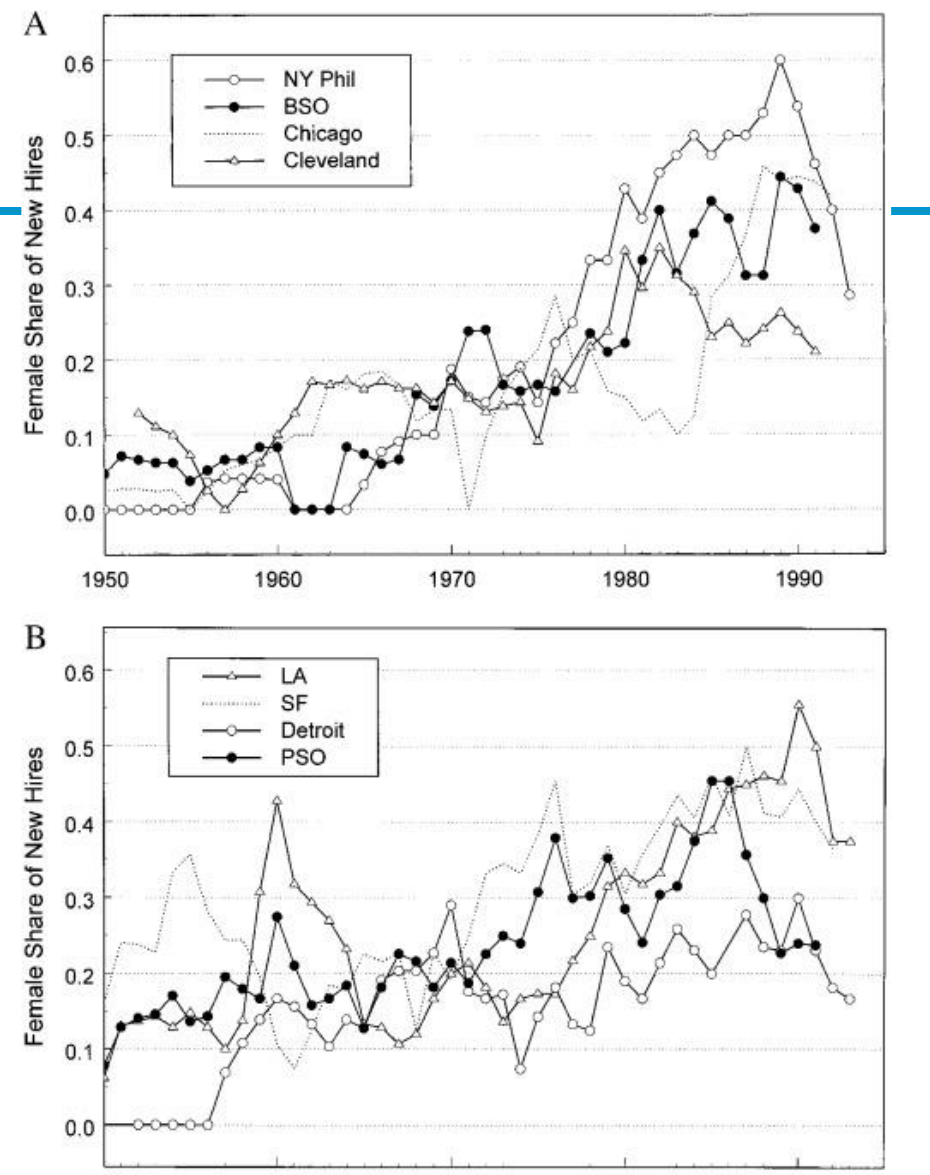
\includegraphics[height=5.1cm]{figures/edu_orchestra_blind_auditions.png}
  \end{center}
  \footnotesize
  US orchestras that introduced \textbf{blind auditions} (candidate plays behind a screen) saw the female share of new hires rise sharply relative to orchestras that didn't --- the screen alone explains roughly one-third of the increase in women's hiring share.\\
  \srcnote{Goldin \& Rouse (2000).}
\end{frame}

\begin{frame}{The Gender Wage Gap}
  \begin{center}
    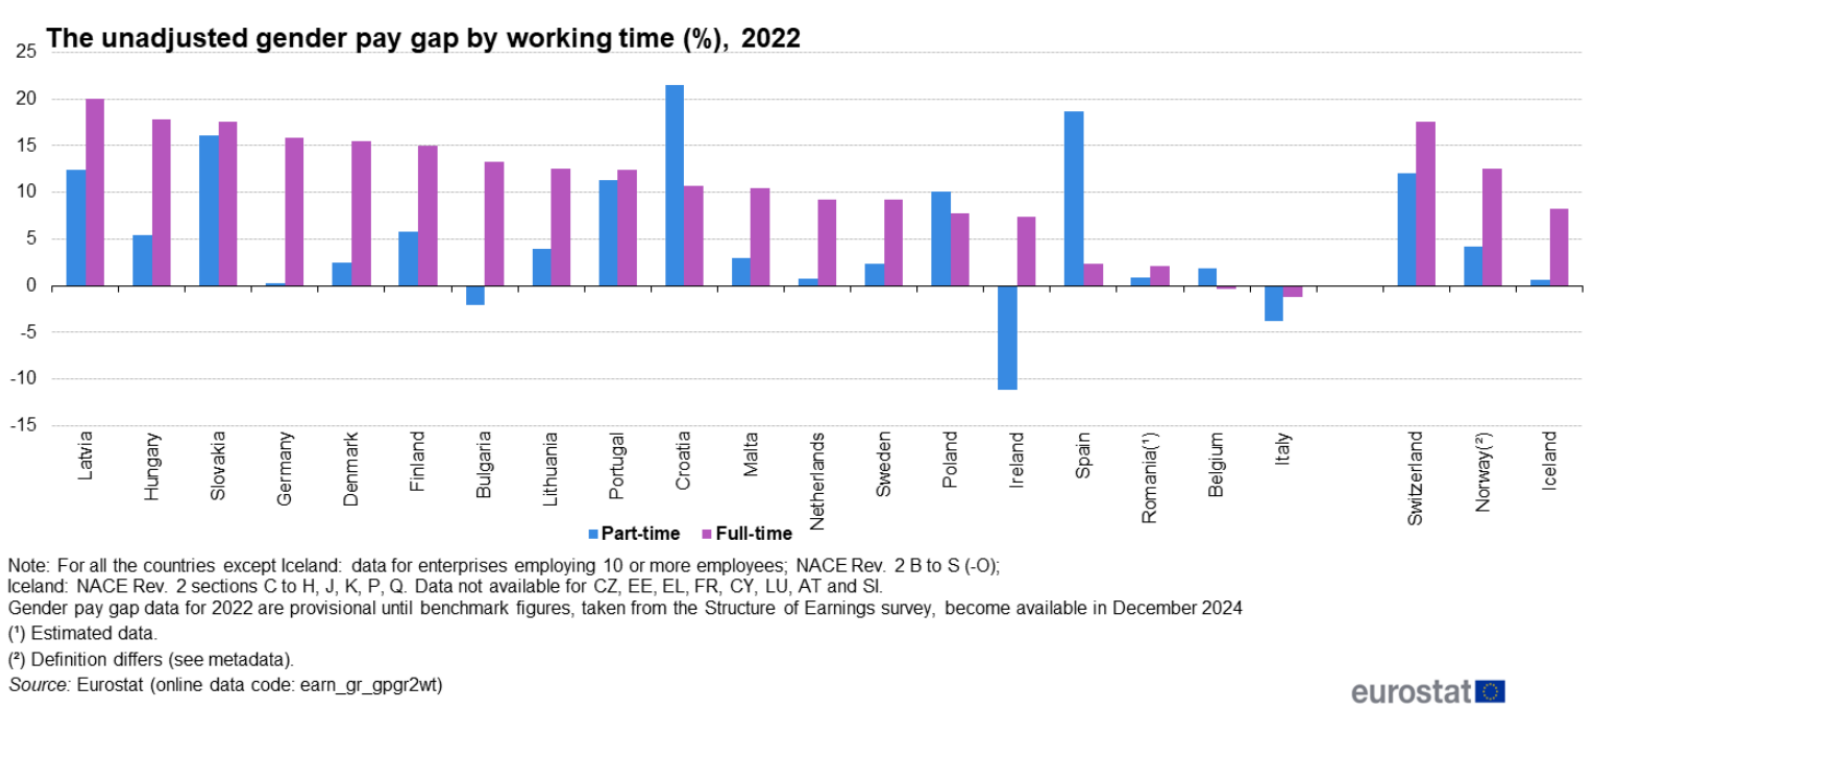
\includegraphics[width=0.85\textwidth]{figures/edu_gender_pay_gap_eu.png}
  \end{center}
  \footnotesize
  The \emph{unadjusted} gender pay gap varies enormously across Europe and by full-time vs.\ part-time status. Part of the gap reflects \textbf{compositional} differences (occupation, hours, seniority) rather than unequal pay for identical work --- the ``adjusted'' gap, controlling for these, is smaller but rarely zero.\\
  \srcnote{Eurostat, 2022.}
\end{frame}

\begin{frame}{Occupational Segregation: Austria}
  \begin{center}
    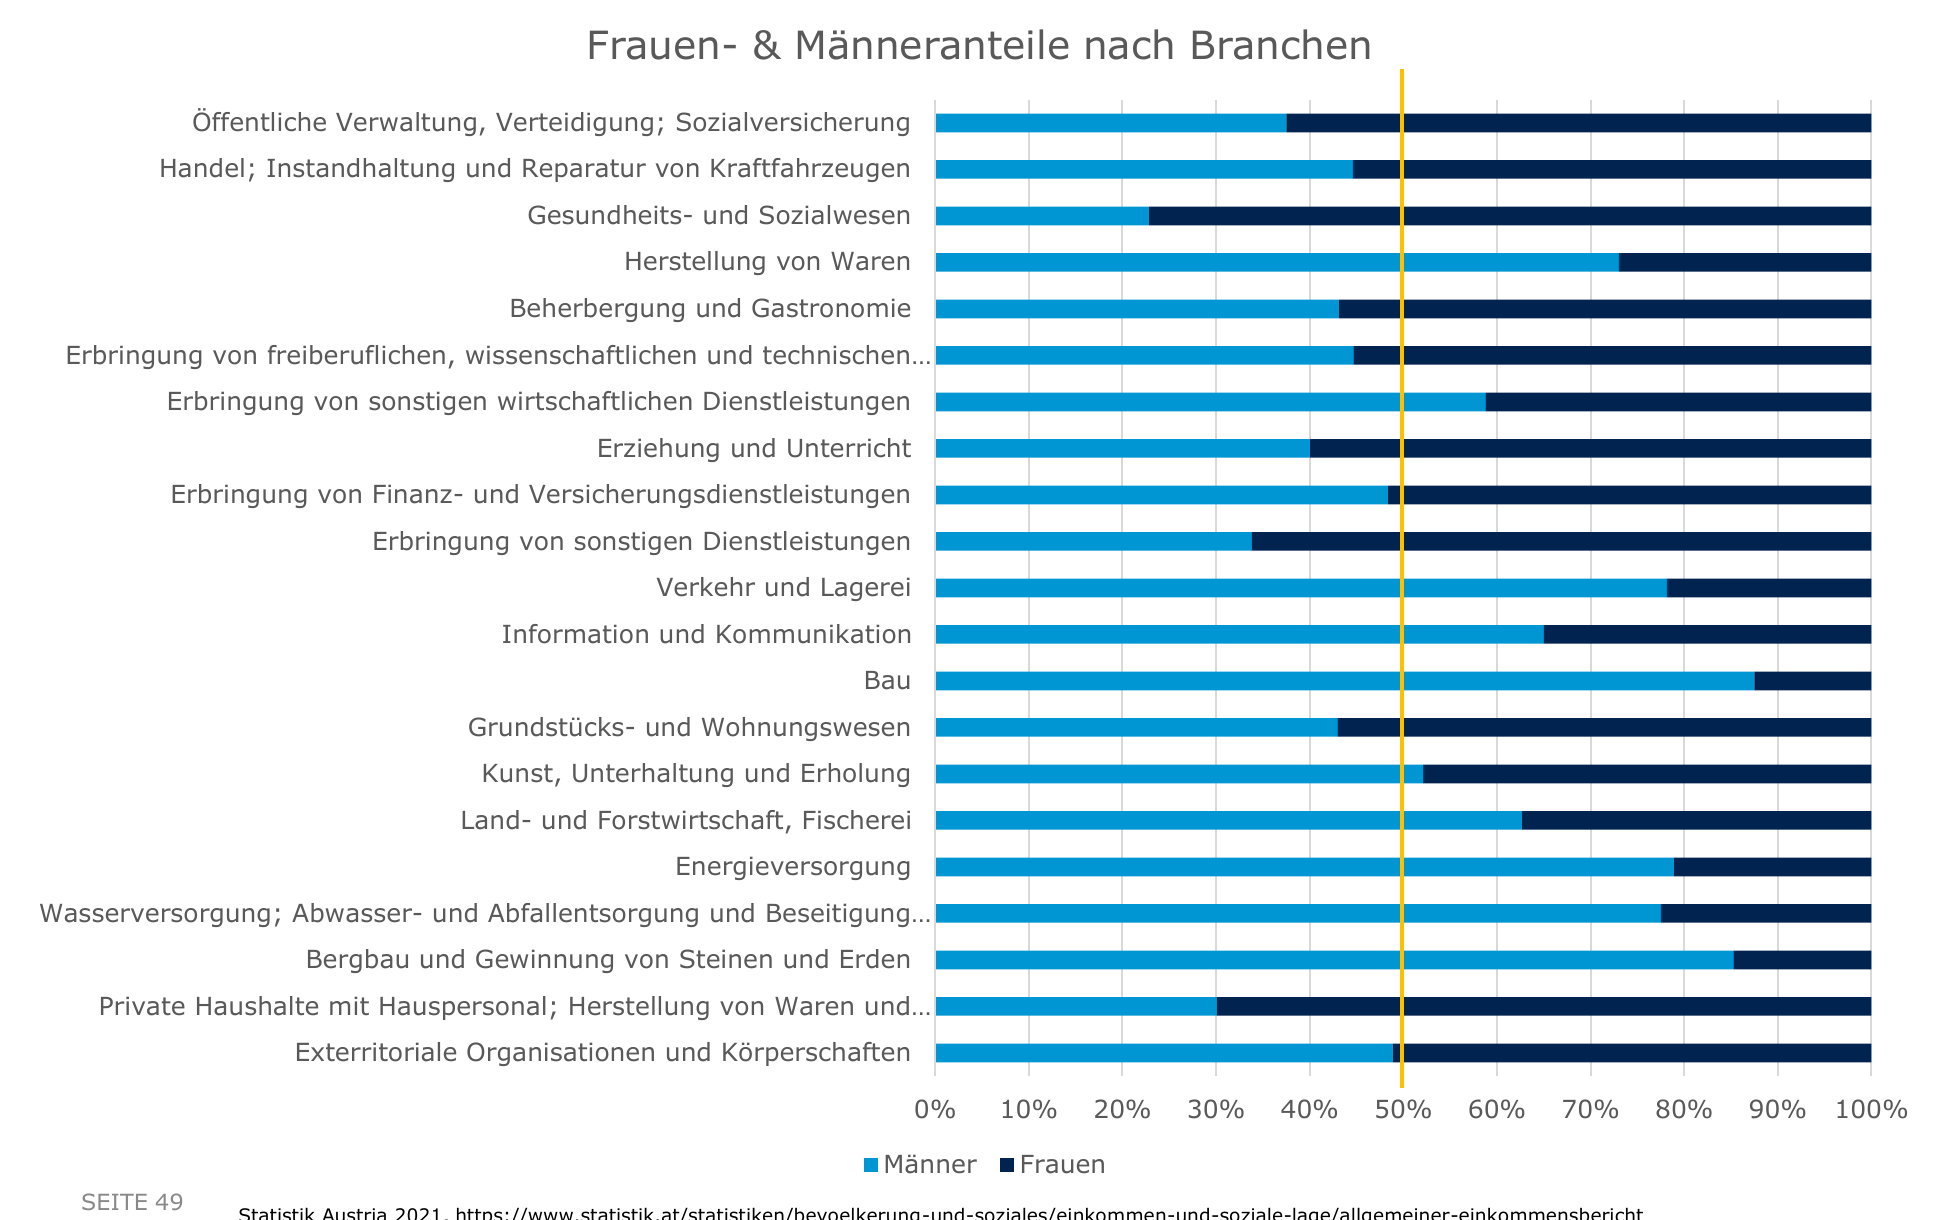
\includegraphics[height=5.0cm]{figures/edu_austria_sector_segregation.png}
  \end{center}
  \footnotesize
  Austrian sectors remain sharply gender-segregated: construction is \(\approx\)90\% male, while health/social work is heavily female-dominated. Segregation matters for tax policy because sectors differ systematically in pay, in benefit generosity, and in exposure to the tax-incidence questions from earlier in this lecture.\\
  \srcnote{Statistik Austria, 2021.}
\end{frame}

\begin{frame}{Child Penalties: Scandinavia and the English-Speaking World}
  \begin{center}
    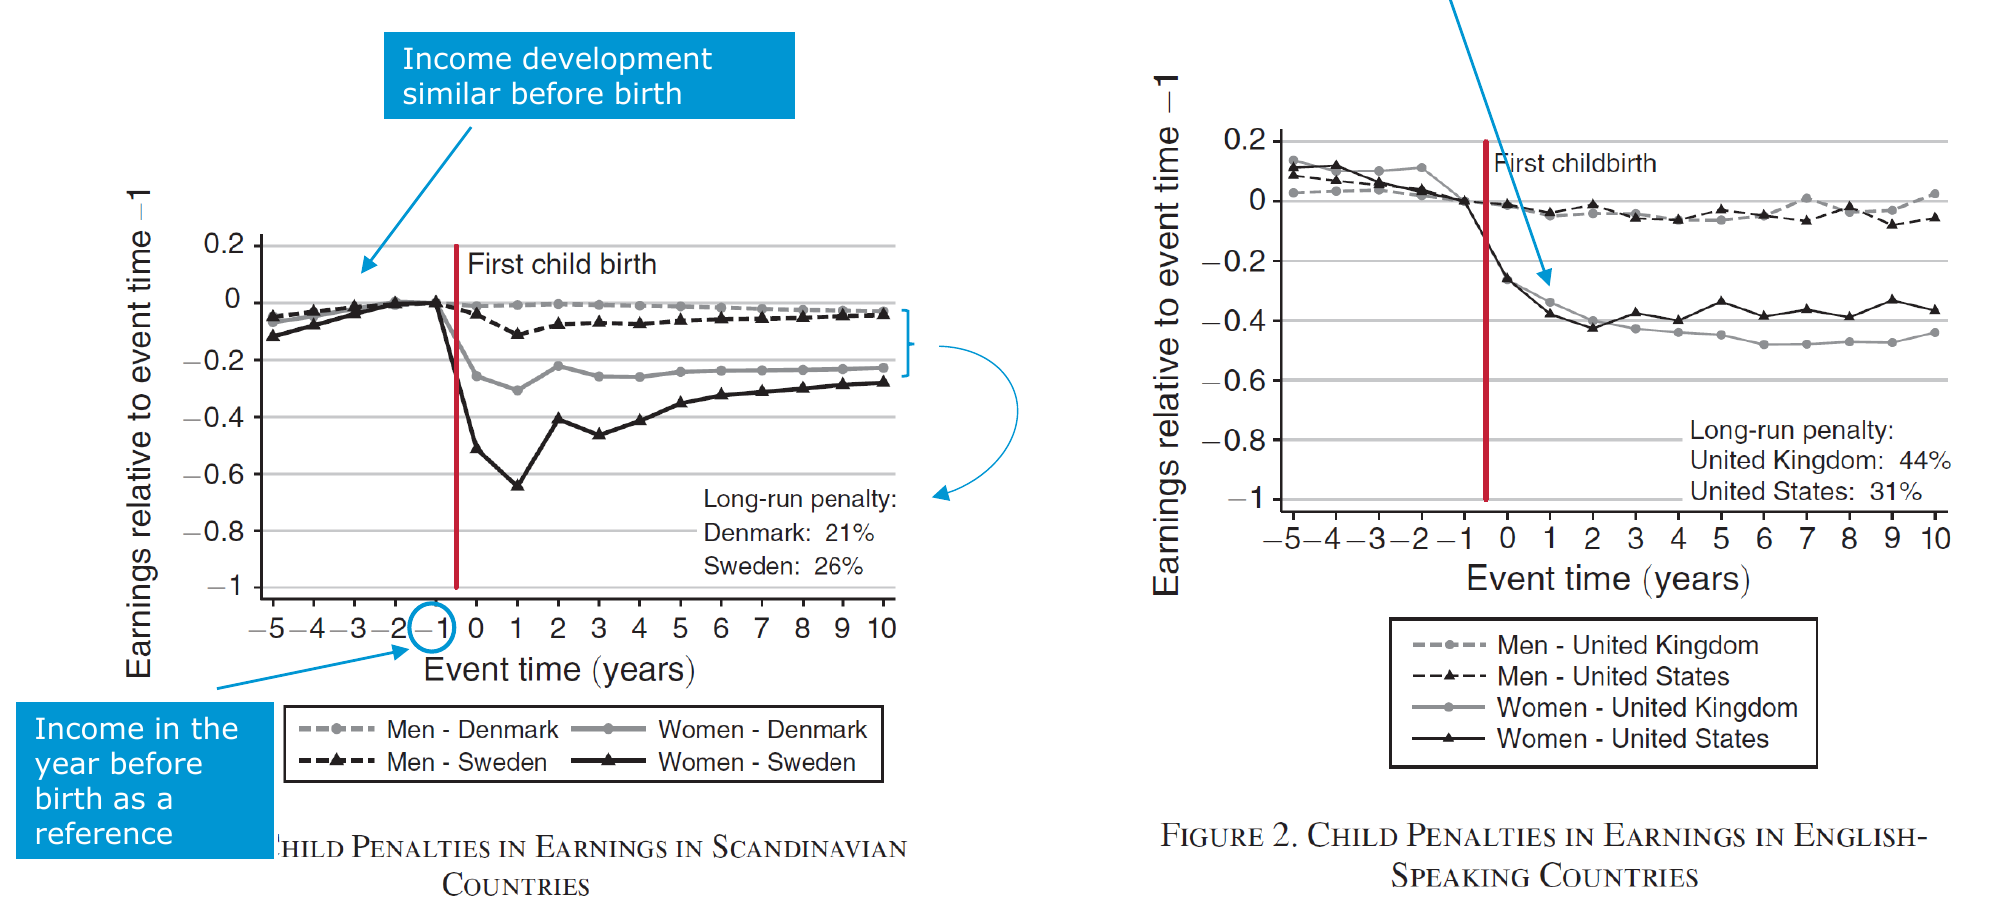
\includegraphics[width=0.82\textwidth]{figures/edu_child_penalty_1.png}
  \end{center}
  \footnotesize
  Women's earnings drop sharply after the first childbirth and never fully recover, while men's earnings are essentially unaffected --- the ``child penalty.'' Long-run penalty: Denmark 21\%, Sweden 26\%, UK 44\%, US 31\%.\\
  \srcnote{Kleven, Landais \& Søgaard (2019).}
\end{frame}

\begin{frame}{Child Penalties: German-Speaking Countries and Gender Norms}
  \begin{center}
    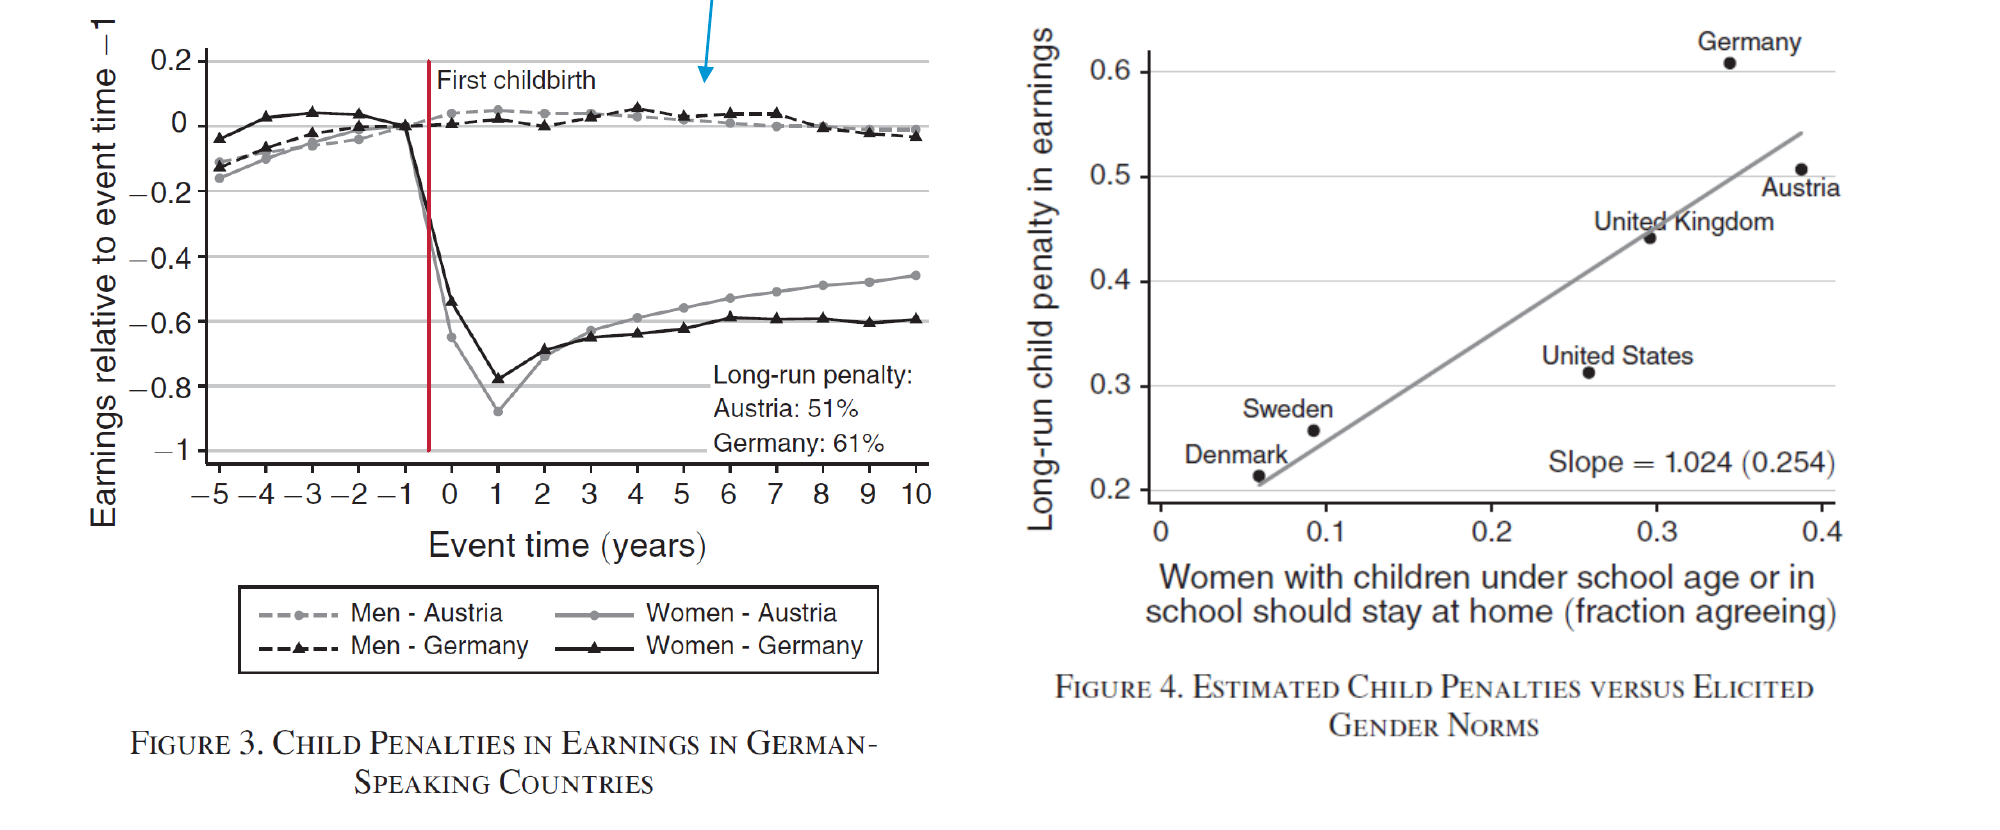
\includegraphics[width=0.82\textwidth]{figures/edu_child_penalty_2.png}
  \end{center}
  \footnotesize
  Austria's long-run child penalty (51\%) is among the \textbf{highest} in the comparison --- second only to Germany (61\%). Right panel: the child penalty correlates strongly with \emph{elicited gender norms} (``women with young children should stay home'') across countries --- suggesting social norms, not just formal tax/transfer design, shape the penalty.\\
  \srcnote{Kleven, Landais \& Søgaard (2019).}
\end{frame}

\begin{frame}{Why This Belongs in a Tax Lecture}
  \small
  \begin{itemize}
    \item The child penalty is a labor-supply response --- and every tax-and-transfer design choice in this lecture (joint vs.\ individual filing, EMTR/participation tax rate, childcare-cost deductibility) changes its \emph{size}, even if it can't eliminate a norms-driven penalty entirely.
    \item Countries with individual taxation \emph{and} extensive public childcare (the Nordics) show smaller child penalties than countries with joint taxation and/or limited childcare support --- consistent with Kleven (2014)'s ``how can Scandinavians tax so much'' argument from earlier in this lecture.
  \end{itemize}
\end{frame}

% =============================================================
\section{The Distribution of the Tax Burden}

\begin{frame}{Who Actually Pays the Taxes?}
  \begin{itemize}
    \item Rather than asking how a \emph{hypothetical} tax change would affect prices (incidence theory), a newer research tradition (Saez \& Zucman, 2019, and successors) asks: given the tax system \emph{as it exists}, what share of everyone's income actually goes to tax, by income rank?
    \item Applied to the Netherlands, Italy, France, and the US, this research finds effective tax rates that \textbf{rise} through the middle of the distribution --- then \textbf{flatten or fall} at the very top.
  \end{itemize}
  \vspace{0.3em}

  The progressivity we build into income-tax \emph{brackets} doesn't automatically show up in the effective rate actually paid, once every tax is counted.
  \
\end{frame}

\begin{frame}{Four Insights on Who Pays}

  \begin{enumerate}
    \setlength{\itemsep}{1pt}
    \item \textbf{Income taxes} are progressive for the bottom 90\% of earners, but play only a minor role at the very top --- where income increasingly comes from capital, not wages.
    \item \textbf{Corporate taxes} act as a kind of minimum tax on the rich, since a large share of top-end income flows through corporate ownership.
    \item \textbf{Consumption taxes} hit lower-income households hardest, because they consume a larger \emph{share} of their income than the wealthy do.
    \item \textbf{Payroll taxes} are levied only on labor income --- and labor income's share of total income \emph{falls} as you move up the distribution, which is regressive.
  \end{enumerate}

\end{frame}

\begin{frame}[fragile]{Try It Yourself: Design Your Own Tax System}
  \small
  Saez \& Zucman built an interactive tool around the same distributional data from the last two slides --- it lets you set tax rates by income group and see the revenue and distributional consequences in real time.
  \vspace{0.5em}
  \begin{center}
    \Large \url{https://taxjusticenow.org/#makeYourOwnTaxPlan}
  \end{center}
  \vspace{0.5em}
  \centering
  \alert{In-class exercise:} pick a distributional goal (e.g.\ ``flat effective rate for everyone'' or ``restore 1950s-style progressivity at the top'') and see what tax rates it actually takes to get there.\\
  \srcnote{Saez \& Zucman, \emph{taxjusticenow.org}, companion site to \emph{The Triumph of Injustice} (2019).}
\end{frame}

% =============================================================
\section{4.6 Capital Taxation}

\begin{frame}{Why Tax Capital Differently from Labor?}
  \small
  \begin{itemize}
    \item So far this lecture has focused on \textbf{labor} income. But capital income (interest, dividends, capital gains, rents) raises distinct questions: it is more \textbf{mobile} across borders, harder to \textbf{observe}, and --- crucially --- taxing it changes not just \emph{how much} people work, but how much they \textbf{save and invest}.
    \item A tax on capital income is, in effect, a tax on \textbf{future} consumption relative to present consumption --- which is why the theory looks quite different from labor-income taxation.
  \end{itemize}
  \srcnote{Gruber, \emph{Public Finance and Public Policy}, Ch.\,22 (Taxation of Capital).}
\end{frame}

\begin{frame}{A Two-Period Model of Saving and Capital Taxation}
  \footnotesize
  An individual earns income $Y$ in period 1, consumes $c_1$, and saves the rest at interest rate $r$ to consume $c_2 = (Y-c_1)(1+r)$ in period 2. Their intertemporal budget constraint:
  \[
    c_1 + \frac{c_2}{1+r} = Y.
  \]
  \vspace{0.3em}
  \begin{itemize}
    \item A tax $t_K$ on \textbf{capital income} lowers the after-tax return to $r(1-t_K)$, tilting the budget line: it is now \emph{more expensive} to consume in period 2 relative to period 1.
    \item This is exactly analogous to a labor-supply tax: it has both a \textbf{substitution effect} (consume more now, save less) and an \textbf{income effect} (you're poorer at any savings level, so save more) --- theoretically ambiguous net effect on saving.
  \end{itemize}
\end{frame}

\begin{frame}{Three Ways to Tax Capital}
  \small
  \begin{itemize}
    \item \textbf{Income tax on capital returns}: taxes interest, dividends, and realized capital gains as they are earned --- the most common approach, and what Austria's \emph{Kapitalertragsteuer} (KESt, 27.5\%) does.
    \item \textbf{Capital gains tax}: taxes the \emph{increase in asset value} only when \textbf{realized} (sold) --- creating a strong incentive to defer selling (``lock-in effect''), unlike an accrual-based tax.
    \item \textbf{Wealth tax}: taxes the \emph{stock} of assets held, regardless of whether they generate income or are sold --- effectively a tax on the \emph{return} an asset is assumed to earn, whether or not it actually does.
  \end{itemize}
\end{frame}

\begin{frame}{The Chamley--Judd Result and Its Critics}
  \footnotesize
  \begin{block}{Chamley--Judd (1985--86)}
    In a standard infinite-horizon growth model, the \textbf{optimal long-run tax rate on capital income is zero} --- any positive capital tax eventually causes unbounded distortion to savings, since the tax compounds every period.
  \end{block}
  \vspace{0.3em}
  \begin{itemize}
    \item Highly influential, but built on strong assumptions: infinite horizons, no heterogeneity in ability to save, no borrowing constraints.
    \item \textbf{Atkinson--Stiglitz (1976)}: capital income should not be taxed \emph{if} labor income can already be taxed optimally (nonlinearly) and preferences are separable between consumption and leisure --- a narrower, more defensible version of the same conclusion.
    \item Modern critiques (heterogeneous returns to savings, borrowing constraints, bequests) substantially weaken the zero-capital-tax result --- most public finance economists today do \emph{not} treat it as a policy prescription.
  \end{itemize}
\end{frame}

\begin{frame}{Does Cutting Capital Taxes Actually Boost Investment? Evidence}
  \begin{center}
    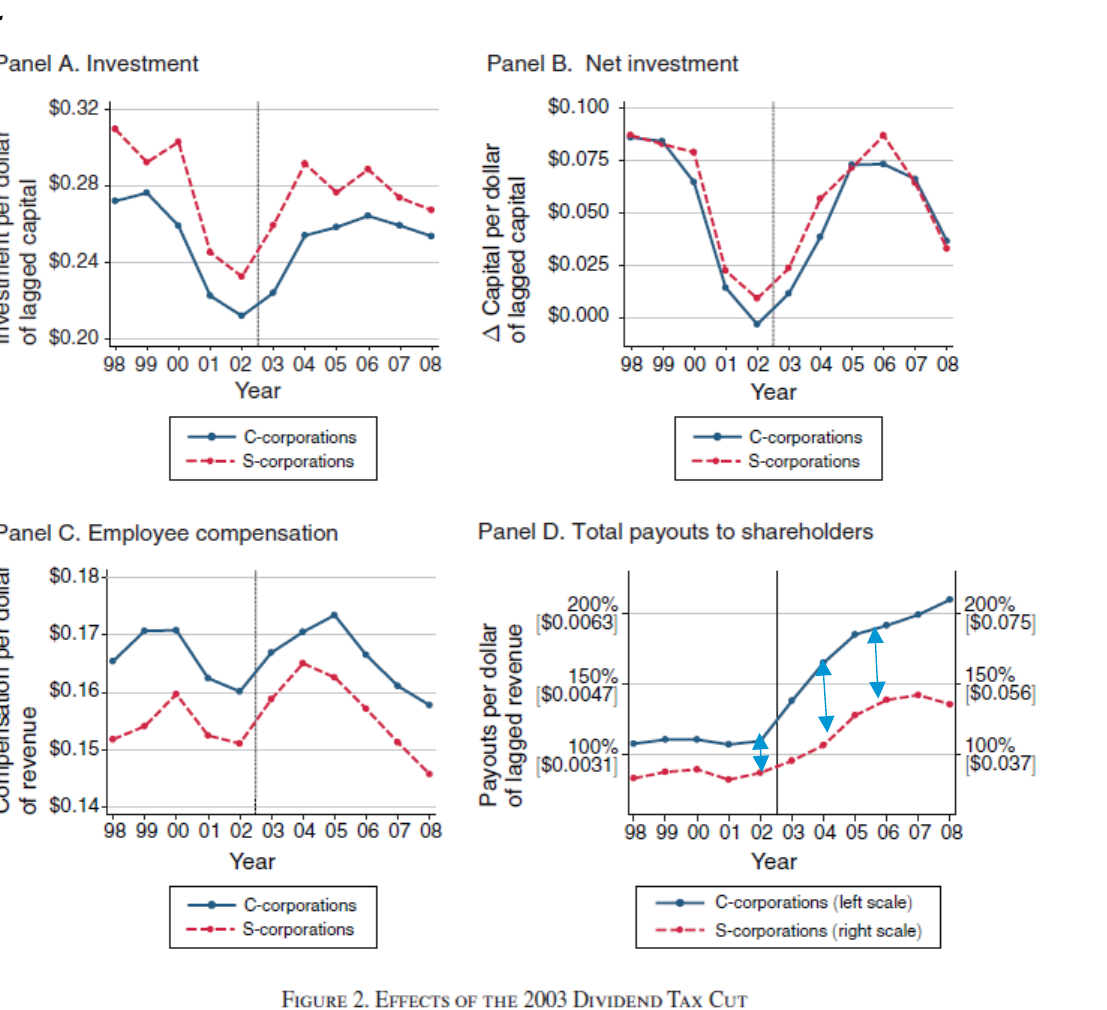
\includegraphics[height=5.0cm]{figures/edu_yagan_dividend_tax.png}
  \end{center}
  \footnotesize
  The 2003 US dividend tax cut (38.5\%$\to$15\%) affected C-corporations but not comparably-taxed S-corporations, a clean control group. Result: \textbf{no detectable effect} on investment or employee compensation (Panels A--C) --- but a clear \textbf{increase in dividend payouts to shareholders} (Panel D). The tax cut redistributed to shareholders without stimulating real economic activity.\\
  \srcnote{Yagan (2015), \emph{Capital Tax Reform and the Real Economy}.}
\end{frame}

\begin{frame}{Wealth Taxation in Europe: A Retreat}
  \begin{center}
    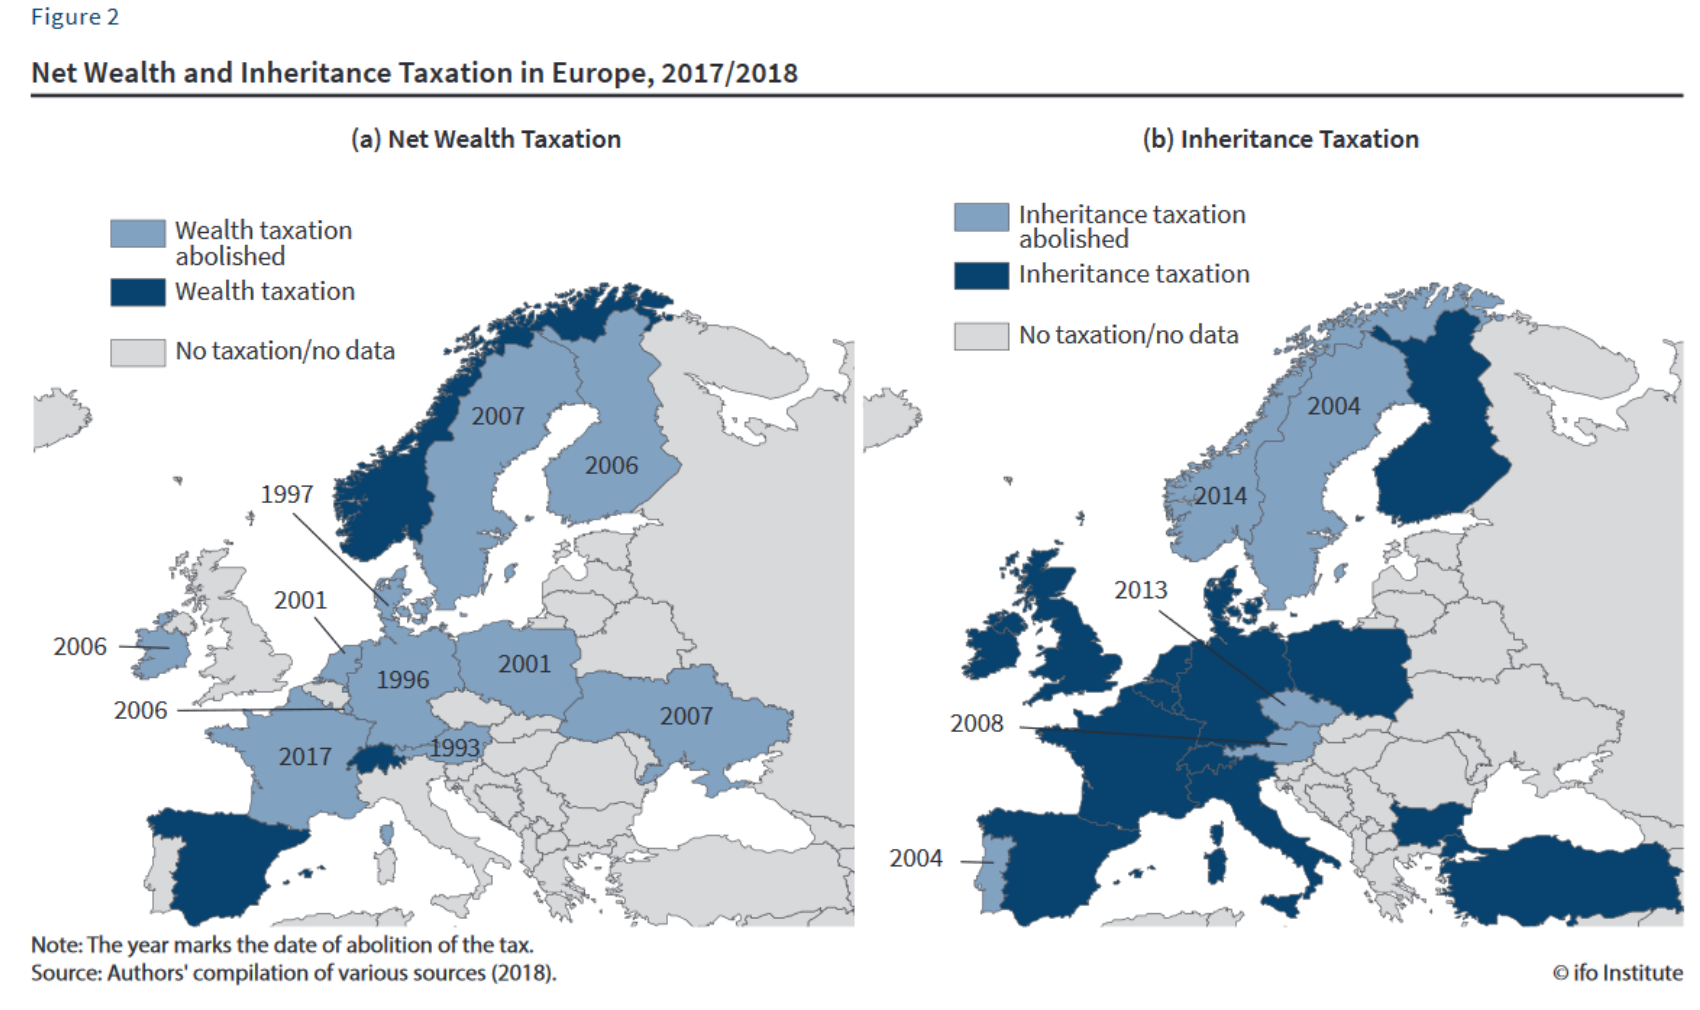
\includegraphics[height=5.2cm]{figures/edu_wealth_tax_abolition_map.png}
  \end{center}
  \footnotesize
  From 12 OECD countries with a net wealth tax in 1990 to just 3 by 2017/18. \textbf{Austria} abolished its wealth tax in 1993 and its inheritance tax lapsed in 2008 (\S4.1) --- part of a broader European pattern, not an isolated choice.
\end{frame}

\begin{frame}{Do Wealth Taxes Actually Reduce Wealth Accumulation? Evidence}
  \begin{center}
    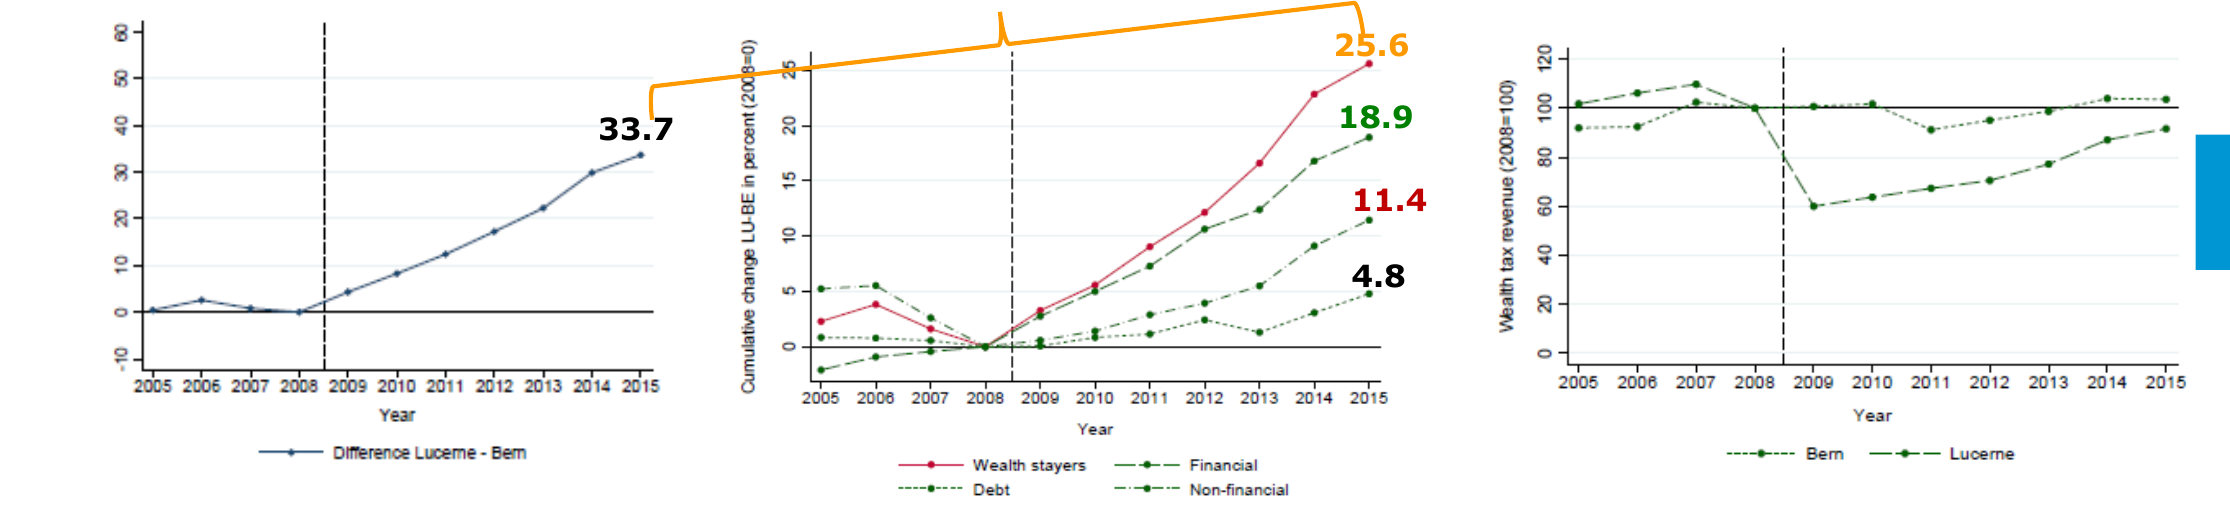
\includegraphics[width=0.85\textwidth]{figures/edu_swiss_wealth_tax_lucerne.png}
  \end{center}
  \footnotesize
  Canton Lucerne cut its wealth tax rate by 50\% in 2009 (Bern, the control, cut by only 14\%). Wealth accumulation in Lucerne rose 33.5 percentage points \emph{more} than in Bern --- driven by migration (24\%), house prices (21\%), and previously-\textbf{underreported} financial assets (49\%) becoming newly worth declaring. Despite this large behavioral response, tax \textbf{revenue still fell} --- no Laffer effect at these rates.\\
  \srcnote{Brülhart et al.\ (2022).}
\end{frame}

\begin{frame}{Global Income and Wealth Inequality}
  \begin{center}
    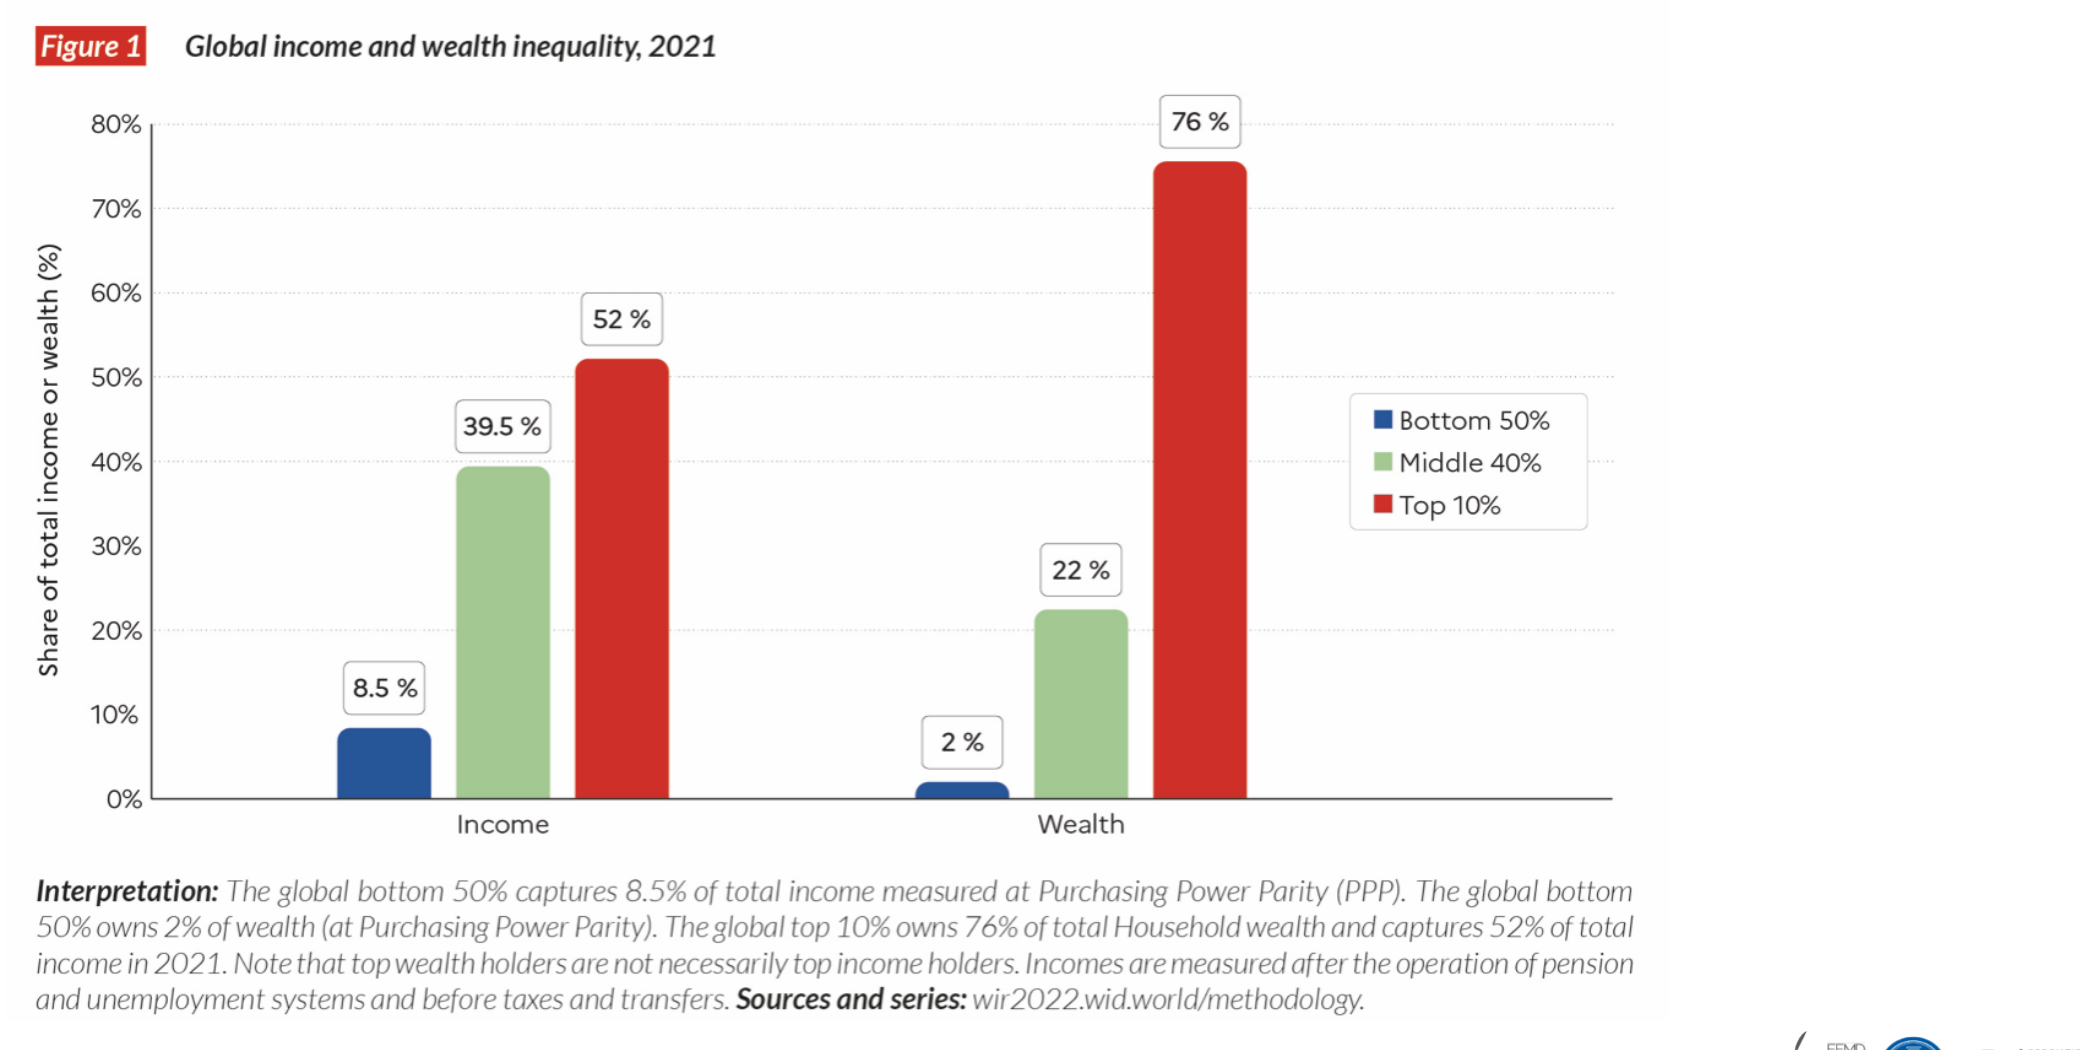
\includegraphics[width=0.68\textwidth]{figures/edu_global_income_wealth_shares.png}
  \end{center}
  \footnotesize
  Globally, the bottom 50\% capture 8.5\% of income but only 2\% of wealth; the top 10\% capture 52\% of income but \textbf{76\%} of wealth. Wealth is \emph{always} more concentrated than income --- the base for a wealth tax is intrinsically less equally distributed than the base for an income tax.\\
  \srcnote{World Inequality Report, 2022.}
\end{frame}

\begin{frame}{Wealth Inequality in Austria I: Lorenz Curves}
  \begin{center}
    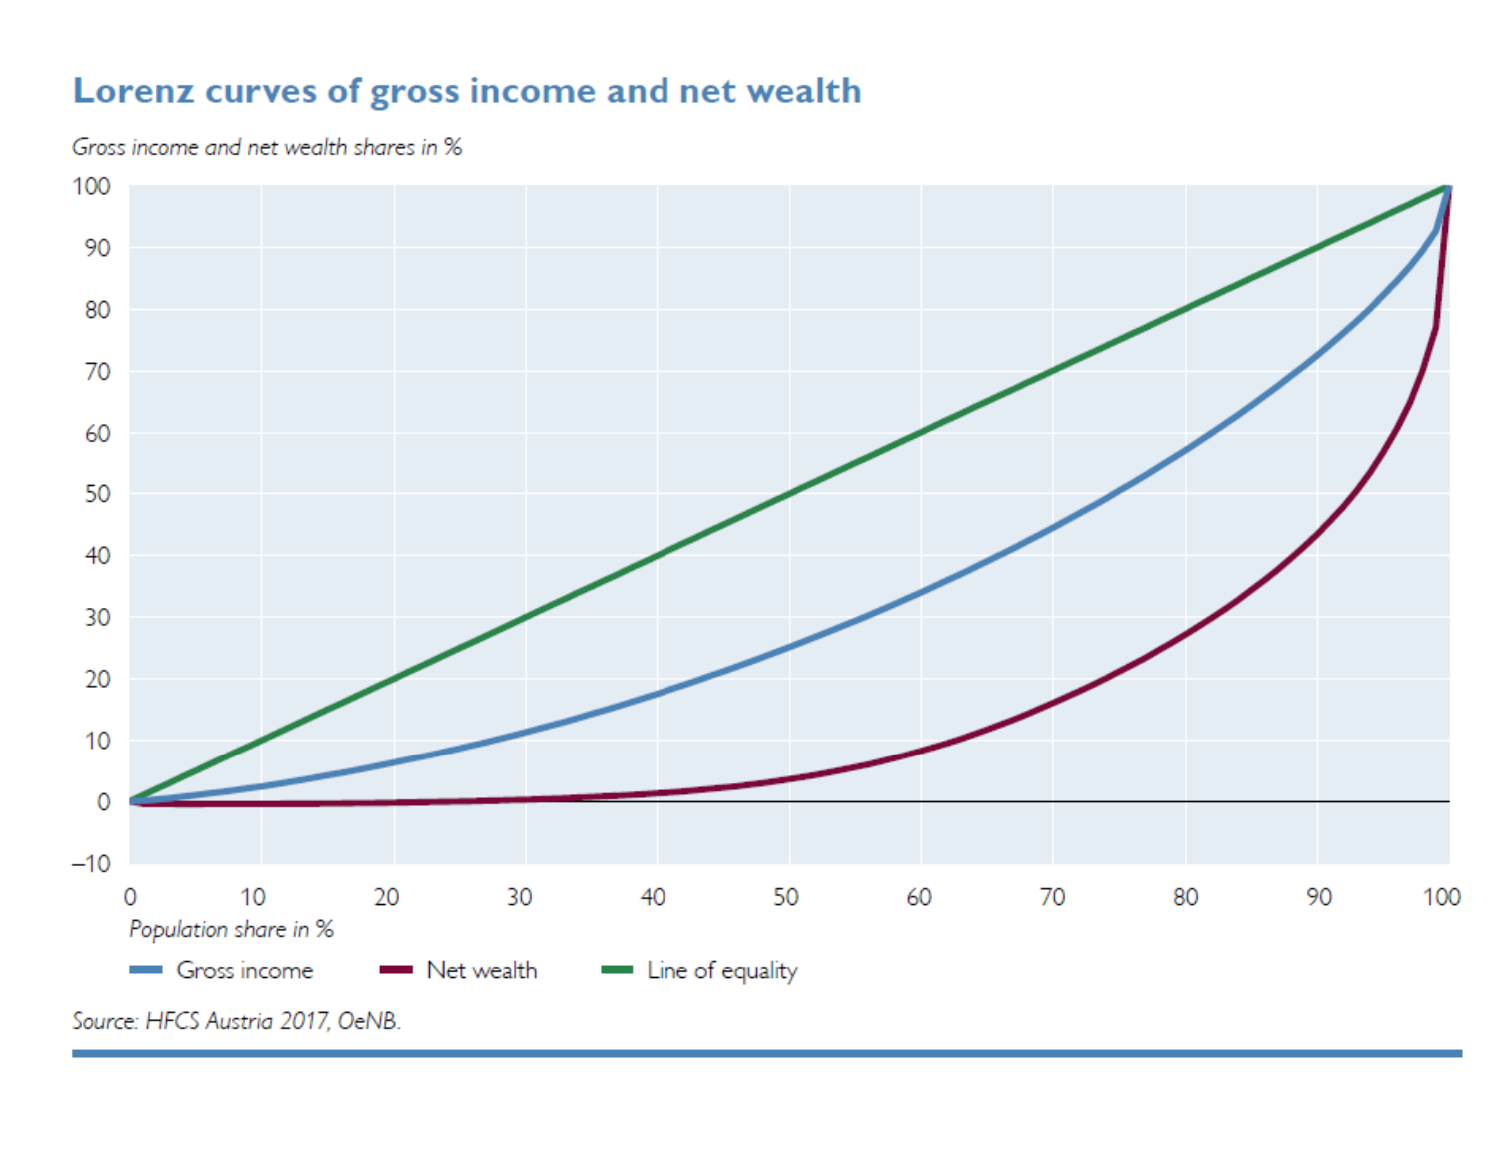
\includegraphics[height=5.1cm]{figures/edu_austria_lorenz_curves.png}
  \end{center}
  \footnotesize
  Austria's top 10\% own just under 30\% of gross income, but over \textbf{50\%} of net wealth; the bottom 50\% together own under 5\% of wealth. Compare to the Gini/Lorenz diagram from Lecture 1 --- this is the same tool applied to \emph{wealth} rather than income.\\
  \srcnote{HFCS Austria 2017, OeNB.}
\end{frame}

\begin{frame}{Wealth Inequality in Austria II: The Full Distribution}
  \begin{center}
    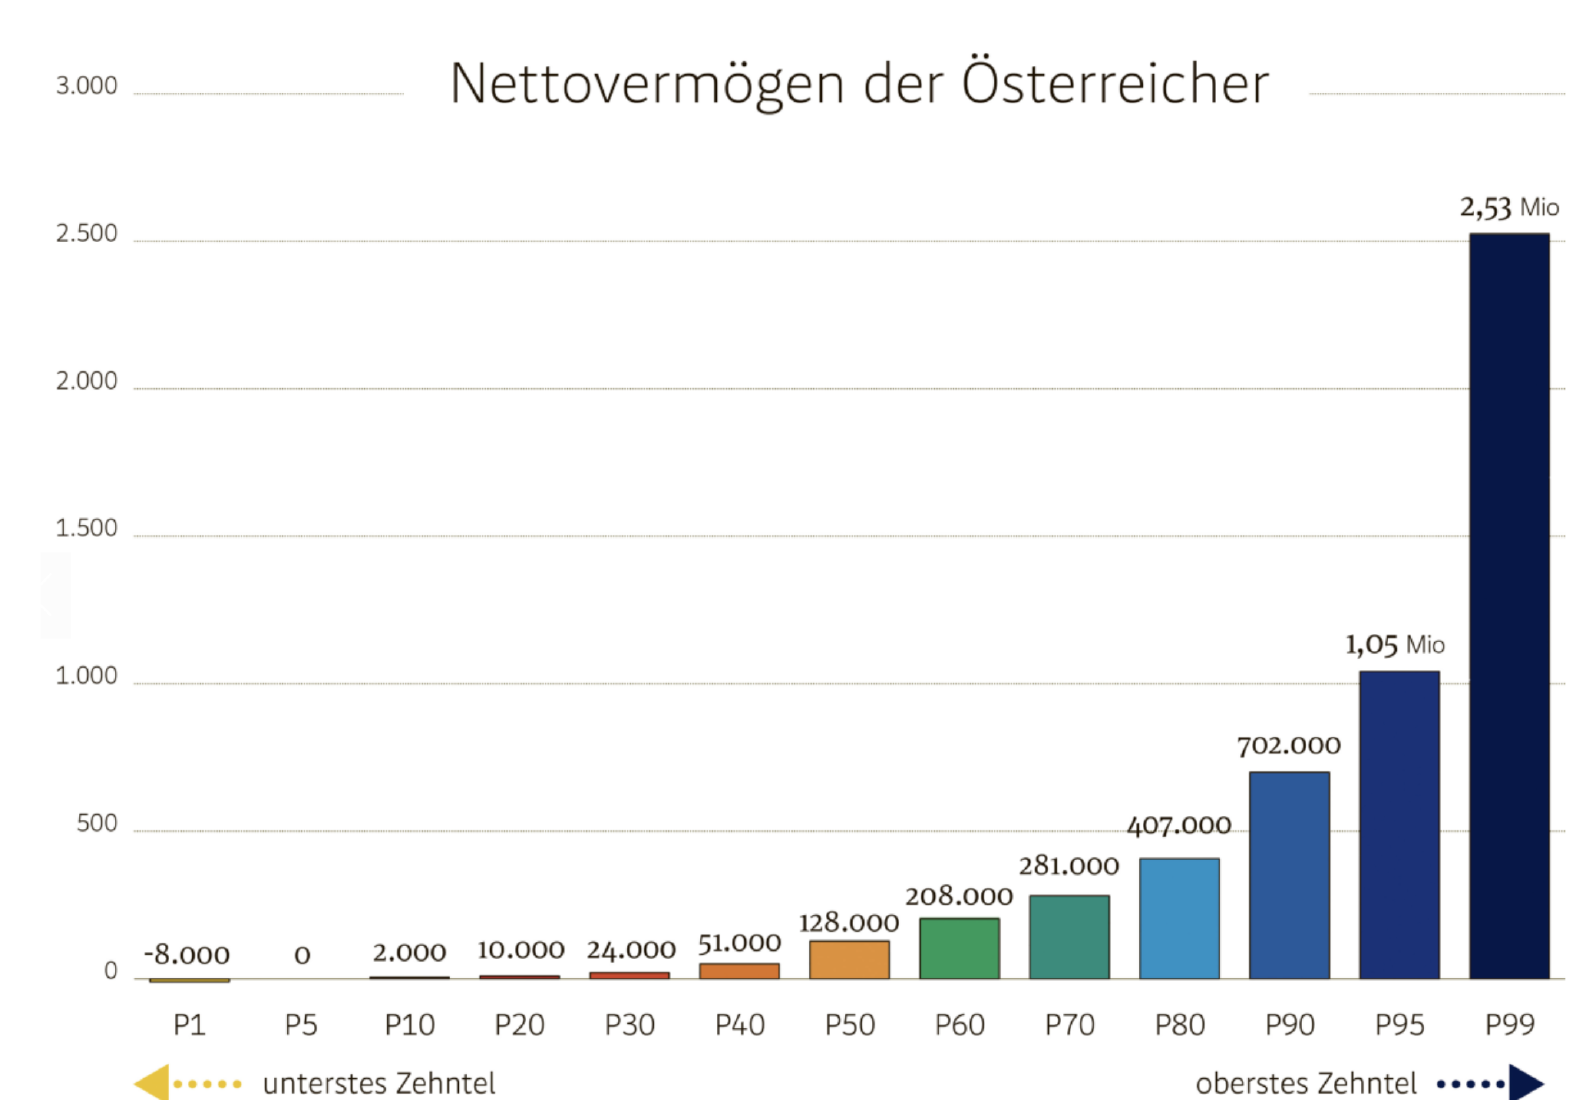
\includegraphics[height=5.1cm]{figures/edu_austria_wealth_percentiles.png}
  \end{center}
  \footnotesize
  Median (P50) net wealth in Austria is \texteuro{}128{,}000; the top percentile (P99) holds \texteuro{}2.53 million --- a 20-fold gap between the median household and the top 1\%. The bottom percentile has \emph{negative} net wealth (more debt than assets).\\
  \srcnote{Nationalbank / Der Standard.}
\end{frame}

\begin{frame}{Wealth at Death: Pen's Parade of Probate Wealth}
  \begin{center}
    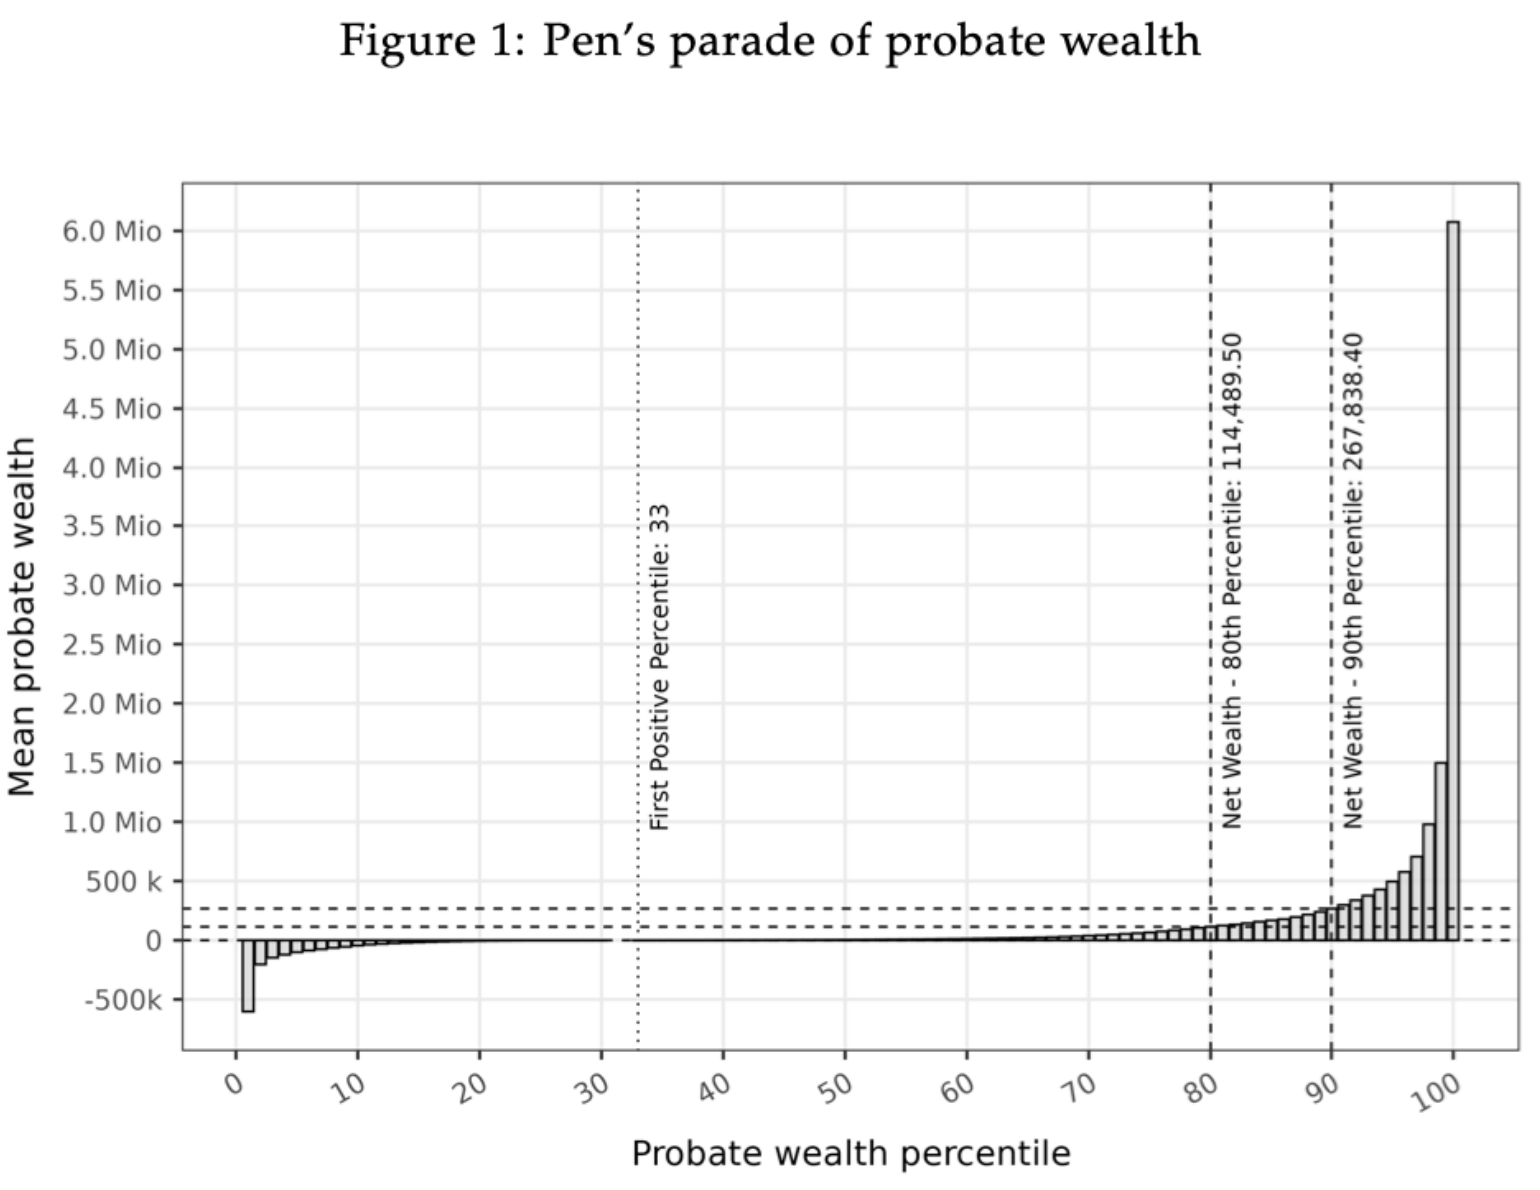
\includegraphics[height=5.1cm]{figures/edu_pens_parade_probate.png}
  \end{center}
  \footnotesize
  The richest 0.1\% of estates leave behind \(\approx\)\texteuro{}22.6 million on average --- while \textbf{30\%} of estates have \emph{negative} net wealth (debts to pharmacies, landlords, collection agencies exceed assets). Over 90\% of total estate wealth is held by the top 10\% of estates --- directly relevant to any inheritance-tax base.
\end{frame}

\begin{frame}{Why Tax Wealth at All? The Functions of Wealth}
  \begin{center}
    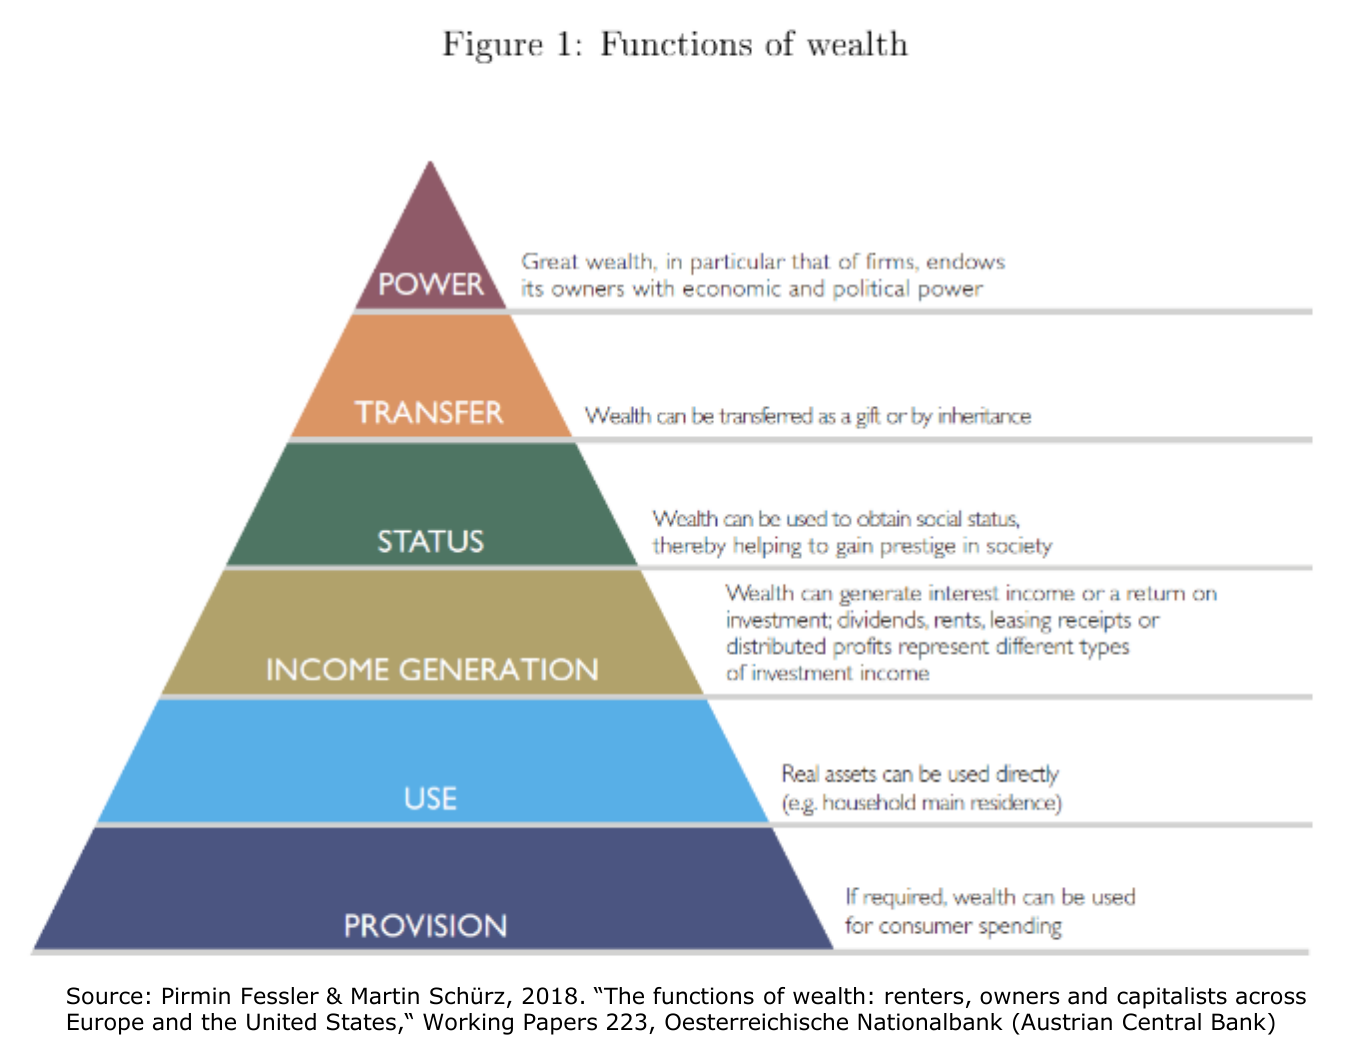
\includegraphics[height=5.0cm]{figures/edu_functions_of_wealth.png}
  \end{center}
  \footnotesize
  Wealth is not just deferred consumption --- it provides \textbf{use} value, \textbf{income}, \textbf{status}, the ability to \textbf{transfer} resources across generations, and ultimately \textbf{power}. The case for taxing wealth (beyond its income) often rests on this last function: very large wealth confers economic and political power independent of the income it generates.\\
  \srcnote{Fessler \& Schürz (2018), Oesterreichische Nationalbank Working Paper 223.}
\end{frame}

\begin{frame}{Capital Taxation: What Should We Conclude?}
  \small
  \begin{itemize}
    \item Implications depend heavily on \textbf{design}: private vs.\ corporate assets, exemptions, progressivity, how the capital tax interacts with the \emph{rest} of the tax system, and the scope for international avoidance.
    \item And on the \textbf{objective}: efficiency, redistribution, fairness/desert (should inherited wealth be taxed differently from earned wealth?), growth, or simply revenue.
  \end{itemize}
  \vspace{0.3em}
  \alert{Discussion:} given everything in this lecture --- incidence, deadweight loss, the Chamley--Judd debate, and Austria's own empirical wealth distribution --- would you reintroduce a wealth or inheritance tax in Austria? What design would you choose?
\end{frame}

% =============================================================




\begin{frame}[standout]
  Thank you!\\
  \vspace{0.5em}
  \small Questions and discussion
\end{frame}

\end{document}
